% H3 report (pdfLaTeX)
\documentclass[11pt,a4paper]{article}
\usepackage[T1]{fontenc}

\usepackage[margin=2.2cm]{geometry}
\usepackage{amsmath,amssymb,amsthm,mathtools,bm}
\usepackage{graphicx,booktabs,tabularx,xltabular,array,enumitem,xcolor}
\usepackage[most]{tcolorbox}
\usepackage{tikz}
\usetikzlibrary{arrows.meta,positioning}
\usepackage[colorlinks,linkcolor=blue!50!black,citecolor=green!35!black,urlcolor=blue!50!black]{hyperref}
\setlist{itemsep=1pt,topsep=2pt}
\numberwithin{equation}{section}
\newtheorem{theorem}{Theorem}[section]
\newtheorem{lemma}[theorem]{Lemma}
\newtheorem{proposition}[theorem]{Proposition}
\newtheorem{corollary}[theorem]{Corollary}
\theoremstyle{definition}
\newtheorem{definition}[theorem]{Definition}
\newtheorem{assumption}[theorem]{Assumption}
\theoremstyle{remark}
\newtheorem{remark}[theorem]{Remark}
\newcommand{\E}{\mathbb E}\newcommand{\R}{\mathbb R}\newcommand{\Z}{\mathbb Z}\newcommand{\Prob}{\mathbb P}
\newcommand{\norm}[1]{\lVert #1\rVert}\newcommand{\abs}[1]{\lvert #1\rvert}\newcommand{\ip}[2]{\langle #1,#2\rangle}
\newcommand{\Dmax}{\Delta_{\max}}\newcommand{\Dcp}{\Delta_{\rm cp}}\newcommand{\Dlow}{\Delta_{\rm low}}
\newcommand{\cN}{\mathcal N}\newcommand{\cA}{\mathcal A}\newcommand{\cG}{\mathcal G}\newcommand{\cF}{\mathcal F}
\newcommand{\Unif}{\mathrm{Unif}}\newcommand{\TV}{\mathrm{TV}}\newcommand{\BC}{\mathrm{BC}}\newcommand{\tmix}{t_{\rm mix}}
\newcommand{\Sph}{\mathbb S^{d-1}}\newcommand{\Ball}{\mathbb B}\newcommand{\iid}{\mathrm{iid}}
\newcommand{\wbar}{\bar\omega}\newcommand{\Atwo}{\cA^{\rm 2pt}_\gamma}
\definecolor{hl}{HTML}{2a78d6}
\tcbset{card/.style={breakable,colback=blue!2,colframe=blue!45!black,boxrule=0.6pt,arc=2pt,left=6pt,right=6pt,top=4pt,bottom=4pt,fonttitle=\bfseries}}

\title{\textbf{H3: independent states ($\tau=1$) --- a two-sided bound\\ and the $\sqrt T$ law for two-point methods}\\[2pt]
\large Local study report}
\author{}
\date{}

\begin{document}
\maketitle
\tableofcontents

%==========================================================================================
\setcounter{section}{-1}
\section{Summary card}\label{sec:card}
\begin{tcolorbox}[card,title={H3 in one page}]
\textbf{Hypothesis.} For independent states ($\tau=1$) and $\gamma\le\gamma_\varepsilon$ the noise threshold of two-point methods of radius $\gamma$ is $\Theta(\varepsilon\gamma\sqrt T/(dR))$; the relevant noise parameter is the oscillation of $\delta$ on the scale $\gamma$, not $\Delta$.

\textbf{Verdict: confirmed in a refined form.} The two-sided bound is proven with explicit constants for the class $\Atwo$ of methods that see only pair differences at radius $\le\gamma$ and draw their directions from laws fixed in advance (adaptive centres, radii, steps, averaging, restarts allowed; this class contains ZO-SGD), for convex $M$-Lipschitz $f$ with $\gamma\le\varepsilon/(4M)$; the smooth class with $\varepsilon/(4M)<\gamma\le\sqrt{\varepsilon/L}$ is not covered by the lower side. Refinements: (i) our upper-bound technique needs a noise law with finite Fisher information (Hellinger instead of KL); the $\pm1$ hash noise proposed in the formulation of the hypothesis (claim H3.2) is decoded exactly for $\Delta>2M\gamma$ on any $f$, and at every $\Delta$ on the linear hypercube (Prop.~\ref{prop:pm1}, E3.5); whether some two-valued noise is hard at the complexity-preserving levels $\Delta\lesssim\sqrt C M\gamma/\sqrt d$ is not decided; (ii) the answer depends on the algorithm class: for arbitrary algorithms we prove only $\Dlow\le\Dmax^E\le71\,\varepsilon\sqrt T/\sqrt d$ (Prop.~\ref{prop:any}); the cited bandit rates, once rescaled to the range of $f$, give a guarantee only at budgets $T\gtrsim C_bd^{k-1}T_0$, so at complexity-preserving budgets $T\asymp CT_0$ they do not beat two-point methods (Cor.~\ref{cor:cross}); the claim ``in the fixed-$\gamma$ class the Bessel part blocks bandit methods'' is \emph{refuted} by a ball-averaging reduction (Prop.~\ref{prop:ballavg}); (iii) both sides hold verbatim with the oscillation $\omega_\delta(2\gamma)/2$ in place of $\Delta$, and the sharp quantity is the mean-square oscillation $\wbar$; the knee of the cost of smooth noise is at $\ell\approx\gamma/\sqrt d$, not $\ell\approx\gamma$ (Lemma~\ref{lem:sin}, E3.2).

\textbf{Main result (one formula).} For i.i.d.\ states with an arbitrary initial law (the protocol of H1), convex $M$-Lipschitz $f$ on $B_R$, $\gamma\le\varepsilon/(4M)$, $\varepsilon<MR/8$ and $T\ge 1+16d^2M^2R^2/((d-1)\varepsilon^2)$ rounds (2 calls each), in the expectation variant
\[
\frac{\varepsilon\gamma\sqrt{T-1}}{4\,dR}\ \le\ \frac{\gamma}{d}\Big(\frac{\varepsilon\sqrt{T-1}}{2R}-\frac{dM}{\sqrt{d-1}}\Big)\ \le\ \Dmax^{E,\mathrm{2pt},\gamma}(\varepsilon;\iid;T)\ \le\ 32\pi\,\frac{\varepsilon\gamma\sqrt T}{dR}
\qquad(\text{Thm.~\ref{thm:main}}).
\]
The lower side is ZO-SGD with batch 1 that idles in round~1 (the state of round 1 has the arbitrary initial law; with a stationary start $T-1$ becomes $T$); no burn-in otherwise. The upper side is one instance (linear $f_v$, rough cell noise with density $\cos^2(\pi t/2)$), lying in the all-radii class and in both readings of (2). Consequences: in the expectation variant $\Dcp^{E}(24)\ge1.034\,M\gamma/\sqrt d$ for $\tau=1$ (H1 had $C=261$, $M\gamma/\sqrt{2d+5}$); separately, the upper side gives $\Dcp^{E,\mathrm{2pt},\gamma}(C)\le32\pi\sqrt C\,M\gamma/\sqrt d$, which closes H1.5d for $\tau=1$ and $\Atwo$.

\textbf{What it implies for the problem.} The case $\tau=1$ is a theorem, not a heuristic: the first branch of H2 at $\tau=1$ holds from both sides \emph{for the class $\Atwo$}; the upper side of the expected picture, $\Dcp\lesssim M\gamma/\sqrt d$ (H1.5d), is proven for this class. For arbitrary query points our bounds leave a gap $\asymp\sqrt d\,MR/\varepsilon$, so the answer depends on which algorithm class $\Dmax$ refers to; for arbitrary algorithms it remains open (\S\ref{sec:contrib}).

\textbf{Numerics} (5 runs each). E3.1 (logistic and $\ell_1$, $d\in\{20,80\}$, $T\le10^6$): collapse in $\Delta/\sqrt T$ confirmed on the progress subsets of the four main problems ($a=0.49$--$0.52$, every CI contains $\frac12$); on all noise-dominated points $a=0.50$--$0.56$, and for both $d=80$ problems the CI excludes $\frac12$ (by $\le0.03$), which meets the criterion ``$a\ne\frac12$'' fixed in the formulation of the hypothesis before this study but not the report's ($a\notin[0.4,0.6]$); errors $\le0.25\times$ the theorem bound. The $\pm1$ sensitivity variant meets the report's refutation criterion ($a=0.67$); at levels with the same $\wbar$ as the Beta runs its all-points fit gives $a=0.52$, but its progress subset ($29$ points) gives $a=0.63\ [0.52,0.77]$, so saturation explains most but not all of the anomaly. E3.2: $\E\|n\|^2\propto1-\Phi_d(2\gamma/\ell)$ to $0.6\%$; in optimisation the cost at $\ell=\gamma$ is $0.18$ ($d=20$) and $0.07$ ($d=80$), not $1$ as predicted by $\min\{1,(\gamma/\ell)^2\}$; factor-2 agreement with $1-\Phi_d$ holds for $d=20$, fails for $d=80$ (saturated design). E3.4 (sanity check only): ZO-SGD never beats the Assouad bound on the hard instance. E3.5: decoded $\pm1$ noise reproduces the noiseless run to $10^{-16}$. E3.3 not run (analytic comparison and plan instead).

\end{tcolorbox}

%==========================================================================================
\section{Place in the global problem}\label{sec:place}
\textbf{Bottleneck closed.} The upper side of the expected picture of the problem statement (its \S3, paragraph ``Expected picture''; the heuristic $\Delta\lesssim M\gamma/\sqrt d$ is stated in its \S1, in the paragraph after the orthogonality condition): $M\gamma/\sqrt d$ was a variance heuristic with no upper bound. H1 proved its lower side ($\Dcp\ge M\gamma/\sqrt{2d+8\tau-3}$) and left the upper side as H1.5d. H3 proves both sides for $\tau=1$ and fixes the algorithm class in which the statement is true. It also bears on the choice of the hard construction: the two-valued law proposed in the formulation of the hypothesis (claim H3.2) is decodable (for $\Delta>2M\gamma$ on any $f$, at every $\Delta$ on the linear hypercube), and our upper-bound technique uses a law with finite Fisher information instead; whether such a law is \emph{necessary} is not shown.

\textbf{Depends on.} The H1 report: Def.~4.19 (protocol, $\Dmax$), Lemma~4.1 (swap of $\E_\pi$, $\E_e$), Lemma~4.3 (ball Stokes identity), Prop.~4.4 (reduction to $m$), Lemma~4.14(a) (Poincar\'e bound $\E\|g_f\|^2\le d^2M^2/(d-1)$), Cor.~4.23 (expectation $\to$ probability). \textbf{Used by.} H2 (its first branch at $\tau=1$ from both sides, for $\Atwo$), H5 (the upper-bound technique for bounded noise), H4 (the $\tau=1$ base case), H7/H10 (rounding as $\tau=1$ noise: the oscillation form, Prop.~\ref{prop:round}).

\begin{figure}[h]\centering
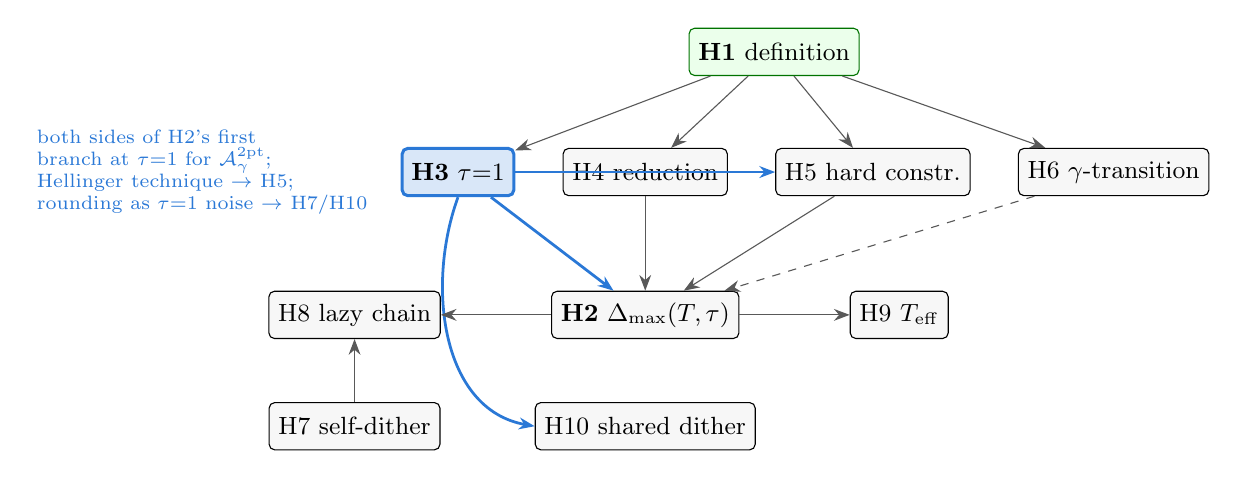
\begin{tikzpicture}[node distance=7mm and 9mm, every node/.style={font=\small},
  h/.style={draw,rounded corners=2pt,minimum width=12mm,minimum height=6mm,fill=gray!6},
  done/.style={h,fill=green!8,draw=green!45!black},
  cur/.style={h,fill=hl!18,draw=hl,line width=1.1pt},
  ar/.style={-{Stealth[length=2mm]},gray!70!black}, dar/.style={ar,dashed}]
\node[done] (H1) {\textbf{H1} definition};
\node[cur,below left=9mm and 22mm of H1] (H3) {\textbf{H3} $\tau{=}1$};
\node[h,right=6mm of H3] (H4) {H4 reduction};
\node[h,right=6mm of H4] (H5) {H5 hard constr.};
\node[h,right=6mm of H5] (H6) {H6 $\gamma$-transition};
\node[h,below=12mm of H4] (H2) {\textbf{H2} $\Dmax(T,\tau)$};
\node[h,right=14mm of H2] (H9) {H9 $T_{\rm eff}$};
\node[h,left=14mm of H2] (H8) {H8 lazy chain};
\node[h,below=8mm of H8] (H7) {H7 self-dither};
\node[h,below=8mm of H2] (H10) {H10 shared dither};
\draw[ar] (H1) -- (H3); \draw[ar] (H1) -- (H4); \draw[ar] (H1) -- (H5); \draw[ar] (H1) -- (H6);
\draw[ar,line width=1pt,hl] (H3) -- (H2); \draw[ar,line width=1pt,hl] (H3) -- (H5); \draw[ar,line width=1pt,hl] (H3.south) to[out=-110,in=170] (H10.west);
\draw[ar] (H4) -- (H2); \draw[ar] (H5) -- (H2);
\draw[ar] (H2) -- (H8); \draw[ar] (H2) -- (H9); \draw[ar] (H7) -- (H8); \draw[dar] (H6) -- (H2);
\node[font=\scriptsize,text=hl,align=left,left=3mm of H3] {both sides of H2's first\\branch at $\tau{=}1$ for $\Atwo$;\\Hellinger technique $\to$ H5;\\rounding as $\tau{=}1$ noise $\to$ H7/H10};
\end{tikzpicture}
\caption{Dependencies between H1--H10 (arrows: ``is used by''). H3 is highlighted; H1 (green) is verified. Thick blue arrows: what H3 delivers.}
\label{fig:diagram}
\end{figure}

%==========================================================================================
\section{Statement and motivation}\label{sec:statement}
\subsection{Definitions}
Notation is that of the global context and of H1: $B_r=\{x:\norm x\le r\}$, $\Ball=B_1$, $e\sim\Unif(\Sph)$, $u,w\sim\Unif(\Ball)$, $d\ge2$; $f$ is convex and $M$-Lipschitz on $B_R$; $f_\gamma(x)=\E_uf(x+\gamma u)$; $T_0=dM^2R^2/\varepsilon^2$. The protocol is Def.~4.19 of H1 with $q=2$: rounds $k=1,\dots,T$, one chain step per round, exogenous chain, both queries of a round in the same state.

\begin{definition}[Independent states]\label{def:iid}
$\cN_\iid(\Delta;\Gamma)$ is the set of noise instances of H1, Def.~4.19(i), whose kernel is $P(s,\cdot)=\pi$ for every $s$. As in H1 the initial law $\nu$ of $s_1$ is arbitrary; then $s_2,s_3,\dots$ are i.i.d.\ $\sim\pi$ and independent of $s_1$, while $s_1\sim\nu$ (``stationary start'' means $\nu=\pi$, i.e.\ all states i.i.d.\ $\sim\pi$). An instance consists of a standard Borel $S$, a jointly Borel $\delta:\R^d\times S\to[-\Delta,\Delta]$, and condition (2) for a.e.\ $x\in B_{R-\gamma'}$ and every $\gamma'\in\Gamma$. $\Gamma=(0,\gamma_0]$ is the recommended all-radii class (equivalently $\E_\pi\delta(x,\cdot)=c$ a.e., H1 Thm.~4.10); $\Gamma=\{\gamma\}$ is the fixed-radius variant. ``$\tau=1$'' in this report means $\cN_\iid$; it is contained in the class $\tmix\le1$ and hence in every $\cN(\Delta,\tau)$.
\end{definition}

\begin{definition}[Two-point methods of radius $\gamma$: the class $\Atwo$]\label{def:class}
An algorithm with $T$ rounds belongs to $\Atwo$ if it has internal randomness $\xi_0$ (drawn once) and fresh independent uniforms $\zeta_1,\zeta_2,\dots$, and in round $t$:
(a) draws a direction $e_t=E_t(\xi_0,\zeta_t)\in\Sph$, so that the law $\mu_t(\xi_0)$ of $e_t$ depends on $t$ and $\xi_0$ only, not on past observations;
(b) chooses a centre and a radius $(y_t,\gamma_t)=Y_t(\xi_0,\zeta_t,e_t,H_{t-1})$ with $\gamma_t\in(0,\gamma]$ and $y_t\pm\gamma_te_t\in B_R$, where $H_{t-1}=(e_s,y_s,\gamma_s,D_s)_{s<t}$;
(c) observes only the difference $D_t=O(y_t+\gamma_te_t,s_t)-O(y_t-\gamma_te_t,s_t)$.
After $T$ rounds it outputs $\hat x=X(\xi_0,H_T)\in B_R$ (all maps Borel). $\Dmax^{\mathrm{2pt},\gamma}$ is $\Dmax$ of H1 Def.~4.19 with the supremum over algorithms restricted to $\Atwo$; superscript $E$ marks the expectation variant.
\end{definition}
$\Atwo$ contains ZO-SGD with any step rule, batching, iterate averaging, restarts, momentum and random query centres; it excludes methods that read individual values (e.g.\ compare $O$ at distant points from different rounds), adaptive choice of the direction law (e.g.\ adaptive coordinate selection), and radii above $\gamma$.

\begin{definition}[Oscillation]\label{def:osc}
$\omega_\delta(2\gamma)=\sup_s\sup_{\norm{y-z}\le2\gamma}\abs{\delta(y,s)-\delta(z,s)}\le2\Delta$ (as in the formulation of the hypothesis), and the mean-square pair oscillation $\wbar(y)^2=\E_{s\sim\pi}\E_e\big[(\delta(y+\gamma e,s)-\delta(y-\gamma e,s))^2\big]$, $\wbar=\sup_{y\in B_{R-\gamma}}\wbar(y)\le\omega_\delta(2\gamma)$.
\end{definition}

\subsection{Claims}
\begin{center}\small
\begin{tabularx}{\textwidth}{@{}lX@{}}
\toprule
H3.1 & Lower bound: ZO-SGD (batch 1, radius $\gamma$, idle in round 1) is $\varepsilon$-accurate in expectation for every $\Delta\le\Dlow(T)=\frac\gamma d\big(\frac{\varepsilon\sqrt{T-1}}{2R}-\frac{dM}{\sqrt{d-1}}\big)_+$; $\Dcp^E(24)\ge M\gamma/\sqrt d$; with $\xi\equiv0$ the heuristic threshold $M\gamma/\sqrt d$ of the expected picture is recovered in order (informal consistency check). \\
H3.2 & Upper bound for $\Atwo$: $\Dmax^{E,\mathrm{2pt},\gamma}\le32\pi\,\varepsilon\gamma\sqrt T/(dR)$ via a hypercube of linear functions and rough cell noise; the $\pm1$ cell noise does \emph{not} give such a bound. \\
H3.3 & The fork: (a) any algorithm, $\Dmax^E\le16\sqrt2\pi\,\varepsilon\sqrt T/\sqrt d$; (b) where bandit rates beat the two-point formula ($MR/\varepsilon\gtrsim\sqrt d$ for $d^3$ rates, and only at budgets $T\gtrsim d^{k-1}T_0$), conditional on cited results; (c) in the fixed-$\gamma$ class the Bessel part does \emph{not} block bandit methods. \\
H3.4 & Oscillation: the noise part of the estimator is $\le d\,\omega_\delta(2\gamma)/(2\gamma)$; H3.1--H3.2 hold with $\omega_\delta/2$ (and $\wbar/2$) in place of $\Delta$; $\Lambda$-Lipschitz noise costs $M\to M+\Lambda$; rounding has $\omega_\delta\le u$, $\wbar\le u/2$, tie $\Leftrightarrow$ signal erased. \\
H3.5 & Numerics: E3.1 collapse in $\Delta/\sqrt T$; E3.2 cost vs scale $\ell$; E3.3 (not run); E3.4 hard instance (sanity check); E3.5 decoding of $\pm1$ noise. \\
\bottomrule
\end{tabularx}
\end{center}
The formulation of the hypothesis, including the predictions and refutation criteria quoted in this report, was fixed before the study.

\subsection{Why it is worth checking; consequences}
$\tau=1$ is the only case of the main formula H2 that can be settled completely now. If the $\sqrt T$ law failed for independent states, H2 would be false. If it holds, the case $\tau=1$ becomes a theorem with constants and the method class in which it is true, and the rest of H2 becomes a question about how $\tau$ enters. The upper side matters most: it is the first rigorous statement that orthogonality \emph{cannot} buy more than $\sqrt T$ for two-point methods, i.e.\ that the expected picture $M\gamma/\sqrt d$ at $T\asymp T_0$ is a real threshold and not an artefact of the variance analysis. If instead some two-point method tolerated more, the expected picture would be a lower bound only, and H2 would need another first branch.

%==========================================================================================
\section{What is known}\label{sec:known}
\begin{center}\small
\begin{tabularx}{\textwidth}{@{}p{2.6cm}Xp{2.5cm}@{}}
\toprule
Item & Statement as used here & Status here\\
\midrule
Two-point rates and minimax lower bounds & Duchi, Jordan, Wainwright, Wibisono, \emph{Optimal rates for zero-order convex optimization: the power of two function evaluations}, arXiv:1312.2139v2: Cor.~1 (rate $RG\sqrt d/\sqrt k$ with sphere directions), Prop.~1 (lower bound $\frac1{12}(1-\frac1q)\frac{GR}{\sqrt k}\min\{d^{1-1/q},k^{1-1/q}\}$ for linear \emph{stochastic} functionals $F(\theta;X)=\ip\theta X$, Gaussian $X$; it says nothing about a deterministic $f$ with $\Delta=0$), Lemma~6 (separation on $\ell_q$ balls), Lemma~7 (KL chain rule for adaptive pairs), Prop.~3 (single-evaluation lower bound $\frac14\min\{d\sigma/\sqrt k,\dots\}$). & used as template; the separation step is re-proved (Lemma~\ref{lem:assouad}); KL is replaced by Hellinger (bounded noise has infinite KL) \\
Assouad / Le Cam & B.~Yu, \emph{Assouad, Fano, and Le Cam} (1997); Le Cam's inequality $P(A)+Q(A^c)\ge1-\TV(P,Q)$. & used, proof included \\
Hellinger for location families & $H^2(p_b,p)\le b^2I(p)/4$ for $\sqrt p$ absolutely continuous with Fisher information $I(p)$ (e.g.\ Ibragimov--Has'minskii, \emph{Statistical Estimation}, Ch.~I); data processing for $f$-divergences; $\TV\le\sqrt{1-\BC^2}$. & re-proved (Lemma~\ref{lem:hell}, \ref{lem:seq}); numerically checked (V3, V4, V7) \\
Minimal Fisher information on $[-1,1]$ & $\cos^2(\pi t/2)$ has $I=\pi^2$, the minimum over densities on $[-1,1]$ (classical; not needed for correctness). & $I=\pi^2$ checked symbolically (V1); minimality not used \\
Adversarial threshold & Pasechnyuk-Vilensky et al.\ arXiv:2306.16371v5, Thm.~III.1, Prop.~IV.1 (as quoted in H1 \S3). & not used in proofs \\
One-point (bandit) methods & Lattimore--Gy\"orgy, COLT 2023, arXiv:2302.05371; Fokkema et al., COLT 2024, arXiv:2406.06506: convex one-point optimisation with upper rates $d^3$--$d^{3.5}\varepsilon^{-2}$ (up to logarithms), with no noise scale. As stated in these papers, the setting is losses with values in $[0,1]$ and conditionally sub-Gaussian noise of constant scale. We give no theorem numbers and have \emph{not} re-checked the theorem statements, settings, constants or logarithms. & used only in the conditional Cor.~\ref{cor:cross}, with the range made explicit (Assumption~(B)); flagged \\
Lipschitz systematic part & Loginov et al.\ arXiv:2610.05517 treat a systematic Lipschitz component (statement not re-checked). & remark only \\
Obtained by us earlier & The H1 report: Lemmas 4.1, 4.3, 4.14(a); Prop.~4.4; Thm.~4.15 and Cor.~4.17 (lower half of H2 with burn-in, $V=2d^2M^2/(d-1)+(2d+8\tau-3)d\Delta^2/\gamma^2$); Cor.~4.23. The variance heuristic behind the expected picture: threshold $M\gamma/\sqrt d$ (\S\ref{sec:place}). & used \\
New in this report & Lemma~\ref{lem:mom}--Prop.~\ref{prop:round}; experiments E3.1, E3.2, E3.4, E3.5; checks V1--V17. & \\
\bottomrule
\end{tabularx}
\end{center}
%==========================================================================================
\section{Theory}\label{sec:theory}
Throughout, $f$ is convex and $M$-Lipschitz on $B_R$, $f^*=\min_{B_R}f$, $d\ge2$, $0<\gamma<R$, the protocol is H1 Def.~4.19 with $q=2$, and the chain has i.i.d.\ states (Def.~\ref{def:iid}).

\subsection{H3.1: the lower bound (an algorithm)}\label{sec:lower}
\emph{Why it should be true, and where the difficulty is.} With i.i.d.\ states every round is a fresh, independent sample of an estimator whose mean is $\nabla f_\gamma$ (H1 Prop.~4.4: the bias at a fixed state averages out over $\pi$), so the method is plain SGD with a bounded second moment, and the only work is to get the second moment with the right constants. In H1 the correlation between states forced a burn-in and the bound $(2d+8\tau-3)d\Delta^2/\gamma^2$; for independent states neither is needed, and the noise enters only through the mean-square pair oscillation. Two subtleties. The a.e.\ reading of (2): the query centre must avoid a null set, which a random centre of radius $\rho>0$ does. The initial law: the protocol lets $s_1$ have an arbitrary law $\nu$, and (2) is an average over $\pi$, so an estimate formed in round~1 can be biased; the method therefore idles in round~1 (or the chain is assumed to start in $\pi$).

\begin{lemma}[One state, one direction]\label{lem:mom}
Let $y\in B_{R-\gamma}$ be a point at which (2) holds at radius $\gamma$, let $e\sim\Unif(\Sph)$ and $s\sim\pi$ be independent and $Y=\frac d{2\gamma}\big(O(y+\gamma e,s)-O(y-\gamma e,s)\big)e$. Then
\[
\text{(a)}\ \ \E Y=\nabla f_\gamma(y),\qquad\text{(b)}\ \ \big(\E\norm Y^2\big)^{1/2}\le\frac{dM}{\sqrt{d-1}}+\frac{d\,\wbar(y)}{2\gamma}\le\frac{dM}{\sqrt{d-1}}+\frac{d\,\omega_\delta(2\gamma)}{2\gamma}\le \frac{dM}{\sqrt{d-1}}+\frac{d\Delta}{\gamma}.
\]
\end{lemma}
\begin{proof}
Write $Y=g_f+n$ with $g_f=\frac d{2\gamma}(f(y+\gamma e)-f(y-\gamma e))e$ and $n=\frac d{2\gamma}(\delta(y+\gamma e,s)-\delta(y-\gamma e,s))e$.
(a) $\E g_f=\frac d\gamma\E[f(y+\gamma e)e]=\nabla f_\gamma(y)$ by $e\mapsto-e$ and the ball Stokes identity for the continuous $f$ (H1 Lemma~4.3(b)). By $e\mapsto-e$ and Fubini (H1 Lemma~4.1; $\delta$ is jointly Borel and bounded), $\E n=\frac d\gamma\E_{s\sim\pi}\E_e[\delta(y+\gamma e,s)e]=0$ by (2) at $y$.
(b) Minkowski's inequality in $L^2$: $(\E\norm Y^2)^{1/2}\le(\E\norm{g_f}^2)^{1/2}+(\E\norm n^2)^{1/2}$. The first term is $\le dM/\sqrt{d-1}$ by H1 Lemma~4.14(a) (Poincar\'e inequality on $\Sph$ applied to $e\mapsto f(y+\gamma e)$; re-checked numerically in V11). Since $\norm e=1$, $\E\norm n^2=\frac{d^2}{4\gamma^2}\E(\delta(y+\gamma e,s)-\delta(y-\gamma e,s))^2=\frac{d^2\wbar(y)^2}{4\gamma^2}$, and $\wbar(y)\le\omega_\delta(2\gamma)\le2\Delta$.
\end{proof}

\paragraph{Algorithm ZO$(T,\gamma,\rho,\eta;t_0)$.} $t_0\in\{0,1\}$ is the number of idle rounds at the start, $N=T-t_0$ the number of steps, $R'=R-\gamma-\rho>0$, $x_1=0$. Rounds $1,\dots,t_0$: no query. Step $i=1,\dots,N$, performed in round $t=t_0+i$: draw $w_i\sim\Unif(\Ball)$, $e_i\sim\Unif(\Sph)$, set $y_i=x_i+\rho w_i$, query $y_i\pm\gamma e_i$ in state $s_t$, form $Y_i=\frac d{2\gamma}D_ie_i$ and $x_{i+1}=\Pi_{B_{R'}}(x_i-\eta Y_i)$. Output $\bar x=\frac1N\sum_{i\le N}x_i$. It belongs to $\Atwo$ (the direction law is $\Unif(\Sph)$; $y_i$ uses fresh randomness and the history; an idle round is a round with an uninformative query, e.g.\ $D_t$ ignored).

\begin{theorem}[Lower bound with explicit constants]\label{thm:lower}
Let $\delta\in\cN_\iid(\Delta;\Gamma)$ with $\gamma\in\Gamma$, let $\rho\ge0$ with $\gamma+\rho<R$, where $\rho=0$ is allowed if (2) holds at radius $\gamma$ for every $x\in B_{R-\gamma}$, and $\rho>0$ otherwise. The pointwise condition holds, in particular, if $\delta(\cdot,s)\in\cG_\gamma$ for every $s$: by H1 Lemma~4.3(b) each $S_{\delta(\cdot,s)}(x)=\frac d\gamma\E_e[\delta(x+\gamma e,s)e]$ is continuous in $x$ and bounded by $\sqrt d\Delta/\gamma$, so $S_m=\E_\pi S_{\delta(\cdot,s)}$ (H1 Lemma~4.1) is continuous by dominated convergence; it vanishes a.e.\ by (2), hence everywhere. Let $t_0=1$ (arbitrary initial law) or $t_0=0$ (stationary start, $s_1\sim\pi$), $N=T-t_0\ge1$, and put
\[
G=\frac{dM}{\sqrt{d-1}}+\frac{d\,\wbar}{2\gamma},\qquad \eta=\frac{R}{G\sqrt N}.
\]
Then ZO$(T,\gamma,\rho,\eta;t_0)$ uses $T$ rounds ($2N$ calls), and
\[
\E f(\bar x)-f^*\ \le\ \frac{RG}{\sqrt{T-t_0}}+2M(\gamma+\rho).
\]
\end{theorem}
\begin{proof}
Let $F(x)=\E_{w,u}f(x+\rho w+\gamma u)$ on $B_{R'}$. $F$ is convex and $M$-Lipschitz, $f\le F\le f+M(\gamma+\rho)$ (Jensen, since $\E[\rho w+\gamma u]=0$; Lipschitz continuity), and $\nabla F(x)=\E_w\nabla f_\gamma(x+\rho w)$ ($f_\gamma\in C^1$ with $\norm{\nabla f_\gamma}\le M$, H1 Lemma~4.3(b); dominated convergence). Let $\cF_{i-1}$ be generated by everything before step $i$ (including $s_1,\dots,s_{t_0+i-1}$). Step $i$ uses the state $s_{t_0+i}$. If $t_0=1$, then $t_0+i\ge2$, and $s_{t_0+i}\sim\pi$ is independent of $\cF_{i-1}$ and of $(w_i,e_i)$, because $P(s,\cdot)=\pi$ makes $s_2,s_3,\dots$ i.i.d.\ $\sim\pi$ and independent of $s_1$, whatever the initial law, and the chain is exogenous. If $t_0=0$, the same holds for $i=1$ because $s_1\sim\pi$ by assumption. (Independence of $s_1$ from the algorithm is not enough when $s_1\not\sim\pi$: Lemma~\ref{lem:mom}(a) needs $s\sim\pi$; see Remark~\ref{rem:lower}(vi).) If $\rho>0$, $y_i$ has a density given $\cF_{i-1}$, so (2) holds at $y_i$ a.s.; if $\rho=0$ it holds everywhere by assumption. By Lemma~\ref{lem:mom}, $\E[Y_i\mid\cF_{i-1}]=\E_w\nabla f_\gamma(x_i+\rho w)=\nabla F(x_i)$ and $\E[\norm{Y_i}^2\mid\cF_{i-1}]\le G^2$.
Let $x'=\Pi_{B_{R'}}x^*$, so $\norm{x_1-x'}\le R'\le R$ and $\norm{x'-x^*}\le\gamma+\rho$. Non-expansiveness of the projection gives $\norm{x_{i+1}-x'}^2\le\norm{x_i-x'}^2-2\eta\ip{Y_i}{x_i-x'}+\eta^2\norm{Y_i}^2$. Taking expectations and using convexity, $2\eta\E[F(x_i)-F(x')]\le2\eta\E\ip{\nabla F(x_i)}{x_i-x'}\le\E\norm{x_i-x'}^2-\E\norm{x_{i+1}-x'}^2+\eta^2G^2$. Summing over $i\le N$, dividing by $2\eta N$ and using Jensen,
$\E F(\bar x)-F(x')\le\frac{R^2}{2\eta N}+\frac{\eta G^2}2=\frac{RG}{\sqrt N}$.
Finally $f(\bar x)\le F(\bar x)$ and $F(x')\le f(x')+M(\gamma+\rho)\le f^*+2M(\gamma+\rho)$.
\end{proof}

\begin{corollary}[The admissible level]\label{cor:lower}
Let $\gamma+\rho\le\varepsilon/(4M)$ with $\rho$ as in Thm.~\ref{thm:lower}, and let the initial law be arbitrary ($t_0=1$). Then every instance with $\wbar/2\le\Dlow(T)$, in particular every $\delta\in\cN_\iid(\Delta;\Gamma)$ with $\Delta\le\Dlow(T)$, is solved to accuracy $\varepsilon$ in expectation in $T$ rounds, where
\begin{equation}\label{eq:Dlow}
\Dlow(T)=\frac\gamma d\Big(\frac{\varepsilon\sqrt{T-1}}{2R}-\frac{dM}{\sqrt{d-1}}\Big)_+ .
\end{equation}
(With a stationary start, $t_0=0$ and $T-1$ may be replaced by $T$ everywhere below.) Hence $\Dmax^{E,\mathrm{2pt},\gamma}(\varepsilon;\iid;T)\ge\Dlow(T)$, and:
\begin{enumerate}[label=(\alph*)]
\item if $T\ge1+16d^2M^2R^2/((d-1)\varepsilon^2)$, then $\Dlow(T)\ge\varepsilon\gamma\sqrt{T-1}/(4dR)$;
\item (expectation variant) if $\varepsilon<MR/8$, then for every $d\ge2$
\[\Dcp^{E}(24)\ge\Dcp^{E,\mathrm{2pt},\gamma}(24)\ge\Dlow(24T_0)=\frac{M\gamma}{\sqrt d}\Big(\sqrt{6(1-1/(24T_0))}-\sqrt{d/(d-1)}\Big)\ge1.034\,\frac{M\gamma}{\sqrt d}\] (V15; without the idle round the factor is $\sqrt6-\sqrt2=1.035$, V9). In the probability variant of the common block the same bound holds at $C=24/\beta^2$: $\Dcp(24/\beta^2)\ge1.034\,M\gamma/\sqrt d$ for $\gamma+\rho\le\beta\varepsilon/(4M)$ and $\beta\varepsilon<MR/8$ (by (d); cf.\ H1 Cor.~4.23(c));
\item in the form given in the formulation of the hypothesis: $G^2\le2d^2M^2/(d-1)+2d^2\Delta^2/\gamma^2\le4dM^2+2d^2\Delta^2/\gamma^2$, so ``$G^2\le c(dM^2+d^2\Delta^2/\gamma^2)$'' holds with $c=4$, and the condition $RG/\sqrt{T-1}\le\varepsilon/2$ is implied by $\Delta\le\frac\gamma d\sqrt{(T-1)\varepsilon^2/(8R^2)-2dM^2}$, a slightly weaker version of \eqref{eq:Dlow};
\item (probability variant) $\Dmax(\varepsilon,\beta;\iid;T)\ge\Dlow(T)|_{\varepsilon\to\beta\varepsilon}$ by Markov's inequality (H1 Cor.~4.23), with $\gamma+\rho\le\beta\varepsilon/(4M)$.
\end{enumerate}
\end{corollary}
\begin{proof}
By Thm.~\ref{thm:lower} with $t_0=1$, $\E f(\bar x)-f^*\le RG/\sqrt{T-1}+\varepsilon/2$, and $RG/\sqrt{T-1}\le\varepsilon/2$ iff $\frac{d\wbar}{2\gamma}\le\frac{\varepsilon\sqrt{T-1}}{2R}-\frac{dM}{\sqrt{d-1}}$, i.e.\ $\wbar/2\le\Dlow(T)$; and $\wbar\le2\Delta$. (a) $\frac{\varepsilon\sqrt{T-1}}{4R}\ge\frac{dM}{\sqrt{d-1}}$ under the condition on $T$. (b) ZO belongs to $\Atwo$, so $\Dcp^E\ge\Dcp^{E,\mathrm{2pt},\gamma}$. At $T=24T_0$, $\frac{\varepsilon\sqrt{T-1}}{2R}=\sqrt dM\sqrt{6(1-1/(24T_0))}$. The factor $\sqrt{6(1-1/(24T_0))}-\sqrt{d/(d-1)}$ increases in $T_0$, and $\varepsilon<MR/8$ gives $T_0=dM^2R^2/\varepsilon^2>64d$; its infimum over $T_0>64d$ and $2\le d\le10^4$ is $1.0349$, attained as $T_0\downarrow128$ at $d=2$ (V15); for $d>10^4$ the factor exceeds $\sqrt6\sqrt{1-1/(1536\cdot10^4)}-\sqrt{1+1/(10^4-1)}>1.4$. Probability variant: at $T=(24/\beta^2)T_0(\varepsilon)=24\,T_0(\beta\varepsilon)$, (d) and the expectation bound at accuracy $\beta\varepsilon$ give the same factor. (c) $(a+b)^2\le2a^2+2b^2$ and $2d^2/(d-1)\le4d$ for $d\ge2$. (d) H1 Cor.~4.23.
\end{proof}

\begin{remark}[Consistency checks and variants]\label{rem:lower}
(i) \emph{Heuristic threshold (informal consistency check, not a proven claim).} With $\xi\equiv0$ (a single state, a deterministic $\delta$ orthogonal to the randomization at every point) and $b=1$, Lemma~\ref{lem:mom} and Cor.~\ref{cor:lower}(b) give admissibility up to $\Delta\asymp M\gamma/\sqrt d$ at $T\asymp T_0$, which matches the order of the variance-heuristic threshold $M\gamma/\sqrt d$ of the expected picture (\S\ref{sec:place}; problem statement, \S1, the paragraph after the orthogonality condition); the heuristic is not derived in this report, and the constants are not compared. (ii) \emph{Batches.} With a batch of $b$ states per step ($T=bN$ rounds) the per-step second moment is $\le M^2+G^2/b$ and the condition becomes $T-1\ge4R^2(bM^2+G^2)/\varepsilon^2$: batching never reduces the number of rounds for $\tau=1$, it only reduces the number of iterations, at a cost $\le2\times$ in $T$ while $b\le G^2/M^2$. (iii) \emph{Enlarged domain.} If $f$ is convex and $M$-Lipschitz on $B_{R+\gamma+\rho}$, queries may leave $B_R$ and the iterate is projected on $B_R$, the projection term disappears and the bound reads $RG/\sqrt T+M(\gamma+\rho)$: then $\gamma=\varepsilon/(2M)$ (the choice in the formulation of the hypothesis) works. (iv) \emph{Mixing time 1 but not i.i.d.} For $\tmix\le1$ chains H1 Cor.~4.17 with $\tau=1$ applies (constant $74.5(2d+5)d$ and a burn-in logarithm); the clean constants above need independence. (v) The theorem uses only $\wbar$, not $\Delta$: see \S\ref{sec:osc}.
(vi) \emph{Why round 1 is skipped.} Without the idle round the proof breaks at step 1 when $\nu\ne\pi$, and not only formally. Take $S=\{\pm1\}$, $\pi$ uniform, $\delta(x,s)=\Delta\,s\,\mathrm{sign}(x_1)$: $\E_\pi\delta\equiv0$, so $\delta$ lies in every class, but for $s_1=+1$ and $y=0$, $\E Y_1=\frac d\gamma\Delta\,\E[\mathrm{sign}(e_1)e]=\frac d\gamma\Delta\,\E\abs{e_1}\,\mathbf e_1$, with $\E\abs{e_1}=\Gamma(\frac d2)/(\sqrt\pi\,\Gamma(\frac{d+1}2))\approx\sqrt{2/(\pi d)}$, i.e.\ a bias $\approx\sqrt{2d/\pi}\,\Delta/\gamma$ (V17: Monte Carlo $72.29\pm0.23$ (95\%) vs.\ exact $72.26$ for $d=20$, $\Delta/\gamma=20$). Using round 1 anyway costs an extra $R\sup\norm b/N\le R\sqrt d\Delta/(\gamma N)$ in the bound (H1 Prop.~4.4(a)) plus the excess of the round-1 second moment over $G^2$; the idle round is simpler and costs $T\to T-1$.
(vii) \emph{Anytime step (used in \S\ref{sec:num}).} With $\eta_i=R/(G\sqrt i)$ instead of a constant step, under the assumptions of Thm.~\ref{thm:lower},
$\E f(\bar x_N)-f^*\le3RG/\sqrt N+2M(\gamma+\rho)$ for every $N$. Proof: the one-step inequality of the proof gives $2\E[F(x_i)-F(x')]\le(D_i-D_{i+1})/\eta_i+\eta_iG^2$ with $D_i=\E\norm{x_i-x'}^2\le(2R')^2\le4R^2$ (both points in $B_{R'}$). By Abel summation, $\sum_{i\le N}(D_i-D_{i+1})/\eta_i\le D_1/\eta_1+\sum_{i=2}^ND_i(1/\eta_i-1/\eta_{i-1})\le4R^2/\eta_N=4RG\sqrt N$, since $1/\eta_i$ is increasing; and $\sum_{i\le N}\eta_iG^2=RG\sum_{i\le N}i^{-1/2}\le2RG\sqrt N$. Hence $\sum_{i\le N}\E[F(x_i)-F(x')]\le3RG\sqrt N$; divide by $N$, use Jensen and finish as in the proof.
\end{remark}

\subsection{H3.2: the upper bound (a hard instance)}\label{sec:upper}
\emph{Why it should be true, and where the difficulty is.} A method in $\Atwo$ sees $D_t=g(y_t,e_t)+\zeta_t$, a difference of $f$ over a segment of length $2\gamma$ plus noise of size $\Delta$. On the hypercube of linear functions $f_v=a\ip vx$, the signal that distinguishes $v_j$ from $-v_j$ in one round is $4\gamma a\abs{e_{t,j}}$, and the directions spread one unit of $\sum_je_j^2$ over $d$ coordinates; Assouad then requires $T\gamma^2a^2/\Delta^2\gtrsim d$ for $d$ coordinates, while the optimisation error is $\asymp aR\sqrt d$: this gives $\Delta\lesssim\varepsilon\gamma\sqrt T/(dR)$. Three difficulties: (1) \emph{bounded} noise: any bounded law shifted by $b$ is not absolutely continuous w.r.t.\ itself, so KL (Duchi et al.\ Lemma~7) is infinite; we use Hellinger distance, which only needs finite Fisher information; (2) \emph{adaptivity} without KL's chain rule: we use a sequential lower bound on the Bhattacharyya coefficient, which needs a per-round bound uniform over histories --- this is where the non-adaptive direction law of $\Atwo$ enters; (3) the \emph{two queries of a round share the state}: if both fell into one cell of the noise, the noise would cancel. Cells of diameter $<2\gamma$ settle this for a fixed radius; adaptive radii are handled by coupling with an idealised oracle (the cell size is chosen after the algorithm: $\forall A\ \exists\delta$).

\begin{definition}[Rough cell noise]\label{def:noise}
Let $p$ be a symmetric probability density on $[-1,1]$, $r>0$, $C_z=\frac r{\sqrt d}(z+[0,1)^d)$ for $z\in\Z^d$ (cubes of diameter $r$) and $z(y)$ the index of the cube containing $y$. State space $S=[-1,1]^{\Z^d}$ with $\pi=p^{\otimes\Z^d}$, i.i.d.\ states with stationary start $s_1\sim\pi$ (an upper bound may fix the initial law, since $\Dmax$ requires success for every initial law), and $\delta_r(y,s)=\Delta\,s_{z(y)}$. The default is $p_\star(t)=\cos^2(\pi t/2)$ on $[-1,1]$, with Fisher information $I(p_\star)=\pi^2$ (V1); the experiments use $p=$ law of $2\,\mathrm{Beta}(3,3)-1$, $I=10$ (V1).
\end{definition}

\begin{lemma}[The instance is admissible]\label{lem:inclass}
(i) $S$ is standard Borel, $\delta_r$ is jointly Borel and $\abs{\delta_r}\le\Delta$. (ii) $\E_\pi\delta_r(y,\cdot)=0$ for every $y$; hence (2) holds at every $x$ and every radius: $\delta_r\in\cN_\iid(\Delta;\Gamma)$ for every $\Gamma$, in both readings, and $\delta_r(\cdot,s)\in\cG_\gamma$. (iii) If $\norm{y-y'}>r$ then $\delta_r(y,s)$ and $\delta_r(y',s)$ are independent under $\pi$, each distributed as $\Delta U$, $U\sim p$; states of different rounds are independent.
\end{lemma}
\begin{proof}
(i) A countable product of standard Borel spaces is standard Borel; $z(\cdot)$ is Borel and $(y,s)\mapsto s_{z(y)}=\sum_z\mathbf 1\{z(y)=z\}s_z$ is a countable sum of measurable functions. (ii) $p$ is symmetric, so $\E s_z=0$; (2) then holds trivially: $\E_\pi\E_e[\delta_r(x+\gamma e,s)e]=\E_e[0\cdot e]=0$. Discontinuities of $\delta_r(\cdot,s)$ lie on the faces of the cubes (countably many hyperplanes), so $\delta_r(\cdot,s)\in\cG_\gamma$ (H1 \S2.1). (iii) Points at distance $>r$ lie in different cubes, whose coordinates are independent under $\pi$.
\end{proof}

\begin{lemma}[Hellinger distance of a shifted bounded law]\label{lem:hell}
Let $p$ be a density on $\R$ such that $\sqrt p$ is absolutely continuous with $I(p)=4\int((\sqrt p)')^2<\infty$, and $H^2(P,Q)=\int(\sqrt{dP}-\sqrt{dQ})^2$, $\BC(P,Q)=\int\sqrt{dP\,dQ}=1-H^2/2$. Then for every $b\in\R$, $\sigma>0$:
(a) $H^2(\mathcal L(\sigma U+b),\mathcal L(\sigma U))\le b^2I(p)/(4\sigma^2)$ for $U\sim p$;
(b) for any Markov kernel $K$, $H^2(KP,KQ)\le H^2(P,Q)$; in particular the law of $\sigma U+b-\sigma U'$, $U'\sim p$ independent, satisfies the bound of (a);
(c) $\TV(P,Q)\le\sqrt{1-\BC(P,Q)^2}$.
For $p_\star$: $\sqrt{p_\star}=\cos(\pi t/2)\mathbf 1_{[-1,1]}$ is absolutely continuous on $\R$ and $I(p_\star)=\pi^2$.
\end{lemma}
\begin{proof}
(a) By scaling it suffices to take $\sigma=1$. With $g=\sqrt p$, $g(t-b)-g(t)=-\int_0^bg'(t-v)\,dv$, so by Cauchy--Schwarz $(g(t-b)-g(t))^2\le\abs b\int_0^{\abs b}g'(t\mp v)^2dv$; integrating in $t$ (Tonelli) gives $H^2\le b^2\int g'^2=b^2I/4$. (b) $H^2$ is an $f$-divergence ($\phi(x)=(\sqrt x-1)^2$), which contracts under Markov kernels (data processing); the map $x\mapsto x-\sigma U'$ is such a kernel. (c) $\TV=\frac12\int\abs{\sqrt p-\sqrt q}(\sqrt p+\sqrt q)\le\frac12\big(\int(\sqrt p-\sqrt q)^2\big)^{1/2}\big(\int(\sqrt p+\sqrt q)^2\big)^{1/2}=\frac12\sqrt{(2-2\BC)(2+2\BC)}$. For $p_\star$: $g=\cos(\pi t/2)$ vanishes at $\pm1$, so it is continuous and piecewise $C^1$, and $4\int_{-1}^1\frac{\pi^2}4\sin^2\frac{\pi t}2dt=\pi^2$. (Quadrature: V3 gives $H^2/(b^2I/4)\le0.9997$ for both densities, and $\le0.36$ for the difference $U-U'$ in the Beta case, V4.)
\end{proof}

\begin{lemma}[Sequential BC bound]\label{lem:seq}
Let $\mathsf P,\mathsf Q$ be the laws of the transcript $(q_1,o_1,\dots,q_T,o_T)$ of the same algorithm, i.e.\ with the same query kernels $a_t(dq\mid h_{t-1})$ and with observation kernels $P_t(do\mid h_{t-1},q)$, $Q_t(do\mid h_{t-1},q)$. If for every $t$ and every history $h_{t-1}$
\[
\int a_t(dq\mid h_{t-1})\,\BC\big(P_t(\cdot\mid h_{t-1},q),Q_t(\cdot\mid h_{t-1},q)\big)\ \ge\ 1-\bar x_t,
\]
and if $\bar x_t\le1$ for all $t$, then $\BC(\mathsf P,\mathsf Q)\ge\prod_{t\le T}(1-\bar x_t)$ and $\TV(\mathsf P,\mathsf Q)\le\sqrt{2\sum_t\bar x_t}$. The TV bound also holds, trivially, if some $\bar x_t>1$. (Without $\bar x_t\le1$ the product bound can fail: $\bar x=(3,3)$ gives a product $4>1$.)
\end{lemma}
\begin{proof}
Choose observation kernels $\nu_t=\frac12(P_t+Q_t)$ and jointly measurable densities $p_t=dP_t/d\nu_t$, $q_t=dQ_t/d\nu_t$ (Doob's measurable Radon--Nikodym theorem for kernels on standard Borel spaces). Then $\mathsf P$ and $\mathsf Q$ have densities $\prod_ta_t\,p_t$ and $\prod_ta_t\,q_t$ w.r.t.\ $\prod_ta_t\,\nu_t$, and
\[\BC(\mathsf P,\mathsf Q)=\int\prod_{t\le T}a_t(dq_t\mid h_{t-1})\sqrt{p_tq_t}(o_t)\,\nu_t(do_t).\]
Integrate out $(q_T,o_T)$ first: the innermost integral equals $\int a_T(dq\mid h_{T-1})\BC(P_T,Q_T)\ge1-\bar x_T\ge0$, uniformly in $h_{T-1}$, and the remaining integrand is non-negative; induct on $T$ (the factor $1-\bar x_T$ must be non-negative to multiply the lower bound of the remaining integral). If all $\bar x_t\le1$, $\prod(1-\bar x_t)\ge1-X$ with $X=\sum\bar x_t$, so by Lemma~\ref{lem:hell}(c) $\TV\le\sqrt{1-(1-X)_+^2}\le\sqrt{2X}$. If some $\bar x_t>1$, then $\sqrt{2X}>1\ge\TV$. (Exact enumeration on 200 random two-round adaptive designs: V7.)
\end{proof}

\begin{lemma}[Separation and Assouad for linear functions]\label{lem:assouad}
For $v\in\{\pm1\}^d$ and $a>0$ let $f_v(x)=a\ip vx$ on $B_R$; $f_v$ is convex, $a\sqrt d$-Lipschitz, $\min_{B_R}f_v=-aR\sqrt d$ at $-Rv/\sqrt d$. (i) For every $\hat x\in B_R$, $f_v(\hat x)-\min f_v\ge\frac{aR}{2\sqrt d}\#\{j:v_j\hat x_j\ge0\}$. (ii) For any algorithm with output $\hat x$, writing $\mathsf P_v$ for the law of the transcript under $f_v$ and $v^{(j)}$ for $v$ with the $j$-th sign flipped,
\[
\max_v\E_v[f_v(\hat x)-\min f_v]\ \ge\ \frac{aR}{4\sqrt d}\sum_{j=1}^d\Big(1-\max_{v}\TV(\mathsf P_v,\mathsf P_{v^{(j)}})\Big).
\]
\end{lemma}
\begin{proof}
(i) Let $W=\{j:v_j\hat x_j\ge0\}$, $i=\abs W$. Then $\ip v{\hat x}\ge\sum_{j\notin W}v_j\hat x_j\ge-R\sqrt{d-i}$ (Cauchy--Schwarz on $d-i$ coordinates), so $f_v(\hat x)+aR\sqrt d\ge aR(\sqrt d-\sqrt{d-i})=aR\,i/(\sqrt d+\sqrt{d-i})\ge aR\,i/(2\sqrt d)$ (V6). (ii) Let $\hat v_j=-1$ if $\hat x_j\ge0$ and $+1$ otherwise; then $\{\hat v_j\ne v_j\}\subseteq\{v_j\hat x_j\ge0\}$. With $V$ uniform on the cube, $\max_v\ge\mathrm{avg}_v$ and (i) give $\max_v\E_v[\cdot]\ge\frac{aR}{2\sqrt d}\sum_j\Prob(\hat v_j\ne V_j)$, and $\Prob(\hat v_j\ne V_j)=\frac12[\mathsf P_{+j}(\hat v_j\ne1)+\mathsf P_{-j}(\hat v_j\ne-1)]\ge\frac12(1-\TV(\mathsf P_{+j},\mathsf P_{-j}))$ by Le Cam's inequality, where $\mathsf P_{\pm j}$ are the averages of $\mathsf P_v$ over $\{v_j=\pm1\}$. Pairing $v$ with $v^{(j)}$ and using convexity of $\TV$, $\TV(\mathsf P_{+j},\mathsf P_{-j})\le\max_v\TV(\mathsf P_v,\mathsf P_{v^{(j)}})$.
\end{proof}

\begin{theorem}[Upper bound for two-point methods of radius $\gamma$]\label{thm:upper}
Let $A\in\Atwo$ use $T$ rounds, let $\Delta>0$, and let $p$ satisfy Lemma~\ref{lem:hell} with $I=I(p)$. Put $a=\min\{M/\sqrt d,\ \sqrt d\,\Delta/(4\gamma\sqrt{IT})\}$. For every $\eta>0$ there are $r>0$ and $v\in\{\pm1\}^d$ such that, on $f_v=a\ip v\cdot$ with noise $\delta_r$ (Def.~\ref{def:noise}),
\[
\E_v[f_v(\hat x)-f_v^*]\ \ge\ \min\Big\{\frac{dR\Delta}{32\gamma\sqrt{IT}},\ \frac{MR}8\Big\}-\eta .
\]
If $A$ uses only radii $\gamma_t\ge\gamma_{\min}>0$, then $r=\gamma_{\min}$ works with $\eta=0$. Consequently, with $p=p_\star$ ($I=\pi^2$):
\begin{enumerate}[label=(\alph*)]
\item $\Dmax^{E,\mathrm{2pt},\gamma}(\varepsilon;\iid;T)\le32\pi\,\varepsilon\gamma\sqrt T/(dR)$ for every $\varepsilon<MR/8$;
\item $\Dmax^{\mathrm{2pt},\gamma}(\varepsilon,\beta;\iid;T)\le64\pi\,\varepsilon\gamma\sqrt T/(dR)$ for $\beta\le1/32$ and $\varepsilon<MR/16$;
\item the same bounds hold for every larger class: all-radii or fixed radius, either reading of (2), any $\tau\ge1$, and they hold for the smooth class as well ($f_v$ is linear).
\end{enumerate}
\end{theorem}
\begin{proof}
\emph{Idealised oracle.} Consider first the oracle that returns $D_t=f_v(y_t+\gamma_te_t)-f_v(y_t-\gamma_te_t)+\Delta(U_t-U_t')=2\gamma_ta\ip v{e_t}+\Delta(U_t-U'_t)$ with $U_t,U'_t\sim p$ independent of each other and of everything else.
\emph{One round.} Fix $\xi_0$, a history and the query $(e_t,y_t,\gamma_t)$. Under $v$ and $v^{(j)}$ the law of $D_t$ is that of $\Delta U-\Delta U'$ shifted by two constants differing by $4\gamma_ta\abs{e_{t,j}}\le4\gamma a\abs{e_{t,j}}$. By Lemma~\ref{lem:hell}(a,b), $H^2\le(4\gamma ae_{t,j})^2I/(4\Delta^2)$, so $\BC\ge1-2\gamma^2a^2Ie_{t,j}^2/\Delta^2$. The direction $e_t$ has law $\mu_t(\xi_0)$ whatever the history, so the hypothesis of Lemma~\ref{lem:seq} holds conditionally on $\xi_0$ with $\bar x_t=2\gamma^2a^2I\,p_{t,j}/\Delta^2$, $p_{t,j}=\int e_j^2\,d\mu_t(\xi_0)$.
\emph{All rounds.} Lemma~\ref{lem:seq} gives $\TV(\mathsf P_v^{\xi_0},\mathsf P_{v^{(j)}}^{\xi_0})\le\sqrt{2X_j(\xi_0)}$, $X_j=\sum_t\bar x_t$, uniformly in $v$; by convexity, $\TV(\mathsf P_v,\mathsf P_{v^{(j)}})\le\E_{\xi_0}\sqrt{2X_j(\xi_0)}$. Since $\sum_jp_{t,j}=\E\norm{e_t}^2=1$, Cauchy--Schwarz over $j$ gives
\[
\sum_j\max_v\TV(\mathsf P_v,\mathsf P_{v^{(j)}})\le\E_{\xi_0}\sqrt{2d\textstyle\sum_jX_j}=\frac{2\gamma a\sqrt{dIT}}{\Delta}.
\]
\emph{Risk.} By Lemma~\ref{lem:assouad}(ii), $\max_v\E_v[f_v(\hat x)-f^*_v]\ge\frac{aR\sqrt d}4\big(1-\frac{2\gamma a\sqrt{IT}}{\sqrt d\Delta}\big)$. If $a=\sqrt d\Delta/(4\gamma\sqrt{IT})$ the bracket equals $\frac12$ and the risk is $\ge aR\sqrt d/8=dR\Delta/(32\gamma\sqrt{IT})$; otherwise $a=M/\sqrt d$, the bracket is $>\frac12$ and the risk is $\ge MR/8$.
\emph{Real oracle (Lemma~\ref{lem:couple} below).} For fixed radii $\ge\gamma_{\min}$ and $r=\gamma_{\min}<2\gamma_t$, the two points of a round are at distance $2\gamma_t>r$, so by Lemma~\ref{lem:inclass}(iii) the real oracle has exactly the idealised law. For adaptive radii Lemma~\ref{lem:couple} gives $\TV(\text{real},\text{ideal})\le\eta/(2MR)$ for small $r$; since $0\le f_v-f_v^*\le2aR\sqrt d\le2MR$ on $B_R$, the risk changes by at most $\eta$.
\emph{Consequences.} (a) If an algorithm achieved $\le\varepsilon<MR/8$ on all instances at level $\Delta>32\pi\varepsilon\gamma\sqrt T/(dR)$, the bound with $\eta$ small enough would exceed $\varepsilon$. (b) If $\Prob(f-f^*\le\varepsilon)\ge1-\beta$, then $\E[f-f^*]\le\varepsilon+2\beta aR\sqrt d$; with $\beta\le1/32$ this contradicts risk $\ge aR\sqrt d/8$ unless $aR\sqrt d/16\le\varepsilon$, i.e.\ $\Delta\le64\pi\varepsilon\gamma\sqrt T/(dR)$; in the case $a=M/\sqrt d$ it contradicts $\varepsilon<MR/16$. (c) Lemma~\ref{lem:inclass}(ii); an i.i.d.\ chain has $\tmix=1\le\tau$; $f_v$ is $0$-smooth.
\end{proof}

\begin{lemma}[Coupling with the idealised oracle]\label{lem:couple}
For $A\in\Atwo$ and $\eta'>0$ there is $r>0$ such that, for every $v$, the transcript laws under the real oracle with $\delta_r$ and under the idealised oracle are within $\eta'$ in total variation.
\end{lemma}
\begin{proof}
Under the idealised oracle $\gamma_t>0$ a.s.\ and $T<\infty$, so $\Prob^{\rm id}_v(\min_t2\gamma_t\le r)\to0$ as $r\downarrow0$ for each of the $2^d$ values of $v$; fix $r$ making all of them $\le\eta'$. Build both processes on one space with the same $\xi_0,\zeta_t$ and states $s_t$, and define the idealised noises in round $t$ as $U_t=s_{t,z(y_t+\gamma_te_t)}$, $U'_t=s_{t,z(y_t-\gamma_te_t)}$ if the two cells differ and $U'_t=$ an auxiliary independent draw otherwise. Given the past, $s_t$ is independent of it, so $(U_t,U'_t)$ are i.i.d.\ $p$ given the past: the idealised process has the correct law. The two observations coincide whenever the cells differ, which holds when $2\gamma_t>r$. Hence the trajectories coincide up to the first round with $2\gamma_t\le r$; this event is determined by the common prefix and has the same probability in both processes, at most $\eta'$.
\end{proof}

\begin{proposition}[The $\pm1$ cell noise is decodable]\label{prop:pm1}
Let $\delta(y,s)=\Delta\eta(z(y),s)$ with $\eta=\pm1$ i.i.d.\ over cells and states (the construction literally proposed in the formulation of the hypothesis, claim H3.2) and cells of diameter $<2\gamma$.
(i) \emph{Any $f$, $\Delta>2M\gamma$.} For every round of a method in $\Atwo$ with $\gamma_t=\gamma$, $g:=f(y+\gamma e)-f(y-\gamma e)$ satisfies $\abs g\le2M\gamma<\Delta$ and $D-g\in\{-2\Delta,0,2\Delta\}$, so $g=D-2\Delta\,\mathrm{round}(D/(2\Delta))$ exactly. Hence ZO-SGD applied to the decoded differences has exactly the noiseless law, and for $\Delta>2M\gamma$ no bound of the form $\Dmax^{\mathrm{2pt},\gamma}\lesssim\varepsilon\gamma\sqrt T/(dR)$ can be derived from this family of noises. The same holds for any noise with values in a lattice $\Delta'\Z$ with $\Delta'>4M\gamma$.
(ii) \emph{The linear hypercube, every $\Delta>0$.} On the family $f_v=a\ip v\cdot$, $v\in\{\pm1\}^d$, of Lemma~\ref{lem:assouad} (with $a$ known, as in any minimax argument over this family), one round with $e\sim\Unif(\Sph)$, centre $0$ and radius $\gamma$ identifies $v$ almost surely, so the output $-Rv/\sqrt d$ has error $0$. Hence this family with $\pm1$ noise gives no upper bound on $\Dmax^{\mathrm{2pt},\gamma}$ at any noise level.
Neither part says anything about other function families at $\Delta\le2M\gamma$, which contains the complexity-preserving levels $\Delta\lesssim\sqrt C\,M\gamma/\sqrt d$ (for $C<4d$); whether a two-valued noise can be hard there is open. A law with finite Fisher information is what \emph{our} technique (Lemma~\ref{lem:hell}) needs; its necessity is not shown.
\end{proposition}
\begin{proof}
(i) $\abs g\le M\norm{2\gamma e}$; $\abs{D-g-2\Delta k}<\Delta$ only for $k=(D-g)/(2\Delta)$, so rounding $D/(2\Delta)$ recovers that integer. Lattice case: same argument with $\Delta'$ in place of $2\Delta$. (V13; E3.5.)
(ii) The two points $\pm\gamma e$ are at distance $2\gamma$, so they lie in different cells and $D=2\gamma a\ip ve+\Delta k$ with $k\in\{-2,0,2\}$. Two candidates $(v,k)\ne(v',k')$ give the same $D$ only if $2\gamma a\ip{v-v'}e=\Delta(k'-k)$. If $v=v'$ this forces $k=k'$; if $v\ne v'$, $\ip{v-v'}e$ has a density (a non-zero linear functional of a uniform point of $\Sph$, $d\ge2$), so each of the finitely many equations holds with probability $0$. Hence $D$ determines $v$ a.s.
\end{proof}

\begin{theorem}[Two-sided bound, $\tau=1$]\label{thm:main}
Let $f$ range over convex $M$-Lipschitz functions on $B_R$, the initial law of the chain be arbitrary (H1 Def.~4.19), $\varepsilon<MR/8$, $\gamma\le\varepsilon/(4M)$ (strict if (2) is only required a.e.\ and the instance is not in $\cG_\gamma$), and $T\ge1+16d^2M^2R^2/((d-1)\varepsilon^2)$. Then
\[
\frac{\varepsilon\gamma\sqrt{T-1}}{4\,dR}\ \le\ \Dlow(T)\ \le\ \Dmax^{E,\mathrm{2pt},\gamma}(\varepsilon;\iid;T)\ \le\ 32\pi\,\frac{\varepsilon\gamma\sqrt T}{dR}.
\]
(With a stationary start, $T-1$ becomes $T$.) Both sides are attained inside $\Atwo$ and inside $\cN_\iid(\Delta;\Gamma)$ for both choices of $\Gamma$: the lower side by ZO with one idle round (with $\rho=\varepsilon/(4M)-\gamma$), the upper side by the instance of Thm.~\ref{thm:upper}, which belongs to the all-radii class and to $\cG_\gamma$. The ratio of the constants is $128\pi\approx402$ (and $64\pi\approx201$ for $T\to\infty$ at fixed other parameters). In the probability variant: $\Dlow|_{\varepsilon\to\beta\varepsilon}\le\Dmax^{\mathrm{2pt},\gamma}(\varepsilon,\beta)\le64\pi\varepsilon\gamma\sqrt T/(dR)$ for $\beta\le1/32$, $\varepsilon<MR/16$.
\end{theorem}
\begin{proof}
Cor.~\ref{cor:lower}(a), Thm.~\ref{thm:upper}(a,b), Cor.~\ref{cor:lower}(d).
\end{proof}

\begin{remark}[What is and is not covered]\label{rem:scope}
(i) \emph{Adaptive direction laws} are excluded only by the proof: the per-round bound must be uniform over histories. With KL one would average $p_{t,j}$ over the mixture of hypotheses (Duchi et al., proof of Lemma~7), but KL is infinite here. We conjecture the bound holds for adaptive directions up to a constant; this remains a hypothesis. (ii) The constant $32\pi$ is not optimised: using $I(U-U')$ instead of $I(U)$ would gain $\sqrt{10/3.63}\approx1.66$ in the Beta case (V14), and $\wbar$ instead of $\Delta$ gains another factor (\S\ref{sec:osc}). (iii) For $T<1+16d^2M^2R^2/((d-1)\varepsilon^2)$ the lower side is not established. We do \emph{not} claim that $\Delta=0$ is unsolvable in $\Atwo$ for $T\ll T_0$: Duchi et al.\ Prop.~1 is a lower bound for stochastic objectives and does not apply to a deterministic $f$, and $\Atwo$ allows adaptive centres and radii with fixed (e.g.\ cyclic coordinate) directions, which in the noiseless case can give exact coordinate differences and plausibly support cutting-plane methods with far fewer than $T_0$ rounds when $MR/\varepsilon\gg\mathrm{poly}(d)$. Nothing is concluded here about H2's second branch $\sqrt{\ln T/d}$ at $\tau=1$. (iv) \emph{Scope in $f$ and $\gamma$.} The lower side covers convex $M$-Lipschitz $f$ with $\gamma\le\varepsilon/(4M)$ (or $\gamma\le\varepsilon/(2M)$ on an enlarged domain, Remark~\ref{rem:lower}(iii)). The hypothesis is stated for $\gamma\le\gamma_\varepsilon$, which for $L$-smooth $f$ is $\sqrt{\varepsilon/L}$; the range $\varepsilon/(4M)<\gamma\le\sqrt{\varepsilon/L}$ for smooth $f$ is not covered by the lower side. The upper side covers it (Thm.~\ref{thm:upper}(c)).
\end{remark}

\subsection{H3.3: the fork with one-point (bandit) methods}\label{sec:fork}
\emph{Why it matters.} Thm.~\ref{thm:main} is a statement about $\Atwo$. For $\tau=1$ and $m=$ const the noise is just centred, independent per query when the queries are in different cells, and methods that read individual values at distant points are not limited by the factor $\gamma/R$. We give a rigorous upper bound valid for all algorithms, a rigorous reduction that disposes of the fixed-$\gamma$ part of the hypothesis, and a conditional comparison.

\begin{proposition}[Upper bound for arbitrary algorithms]\label{prop:any}
For any algorithm in the protocol with $q$ queries per round (arbitrary points of $B_R$, individual values observed, adaptive), every $\Delta>0$ and $p$ as in Lemma~\ref{lem:hell},
$\max_v\E[f_v(\hat x)-f_v^*]\ge\min\{\sqrt d\Delta/(16\sqrt{qIT}),\,MR/8\}-\eta$ on the instance of Def.~\ref{def:noise} with $a=\min\{M/\sqrt d,\Delta/(2R\sqrt{qIT})\}$. Hence $\Dmax^E(\varepsilon;\iid;T)\le16\sqrt{qI}\,\varepsilon\sqrt T/\sqrt d$; for $q=2$, $p=p_\star$: $16\sqrt2\pi\,\varepsilon\sqrt T/\sqrt d\approx71.1\,\varepsilon\sqrt T/\sqrt d$ (for $\varepsilon<MR/8$).
\end{proposition}
\begin{proof}
Idealised oracle: distinct points of a round get independent noises $\Delta U$, equal points equal noises (a repeated point carries no extra information). The observations of a round are $q'\le q$ independent shifted copies; the shift between $v$ and $v^{(j)}$ at a point $y$ is $2a\abs{y_j}\le2aR$, so $1-\BC_t\le\frac12\sum_iH_i^2\le\frac q2\frac{(2aR)^2I}{4\Delta^2}=\frac{qa^2R^2I}{2\Delta^2}$ uniformly ($\BC$ of a product is the product, and $\prod(1-c_i)\ge1-\sum c_i$). Lemma~\ref{lem:seq}: $\TV\le aR\sqrt{qIT}/\Delta$ for every $j$. Lemma~\ref{lem:assouad}: risk $\ge\frac{aR\sqrt d}4(1-aR\sqrt{qIT}/\Delta)$; choose $a$ as stated. The coupling of Lemma~\ref{lem:couple} applies with the event ``two distinct points of a round at distance $\le r$'', whose idealised probability tends to $0$ as $r\downarrow0$.
\end{proof}

\begin{proposition}[Ball averaging: the Bessel part does not block one-point methods]\label{prop:ballavg}
Let $\delta\in\cN_\iid(\Delta;\{\gamma\})$ (fixed radius, reading (A)) and let $c$ be the constant with $\hat m_\gamma\equiv c$ (H1 Prop.~4.4(b); it holds at \emph{every} point). For $x\in B_{R-\gamma}$ let $\tilde O(x)=O(x+\gamma u,s)$ with $u\sim\Unif(\Ball)$ fresh and $s\sim\pi$ the state of the round (any round $\ge2$, or round 1 under a stationary start; as in Thm.~\ref{thm:lower}, round 1 is left idle otherwise). Then $\E\tilde O(x)=f_\gamma(x)+c$ for every $x$, $\abs{\tilde O(x)-f_\gamma(x)-c}\le2M\gamma+2\Delta$, and the errors of different rounds are independent given the query points. Consequently any algorithm for convex optimisation with a one-query-per-round oracle whose noise is conditionally independent, zero-mean and bounded by $\sigma$, run on $f_\gamma$ over $B_{R-\gamma}$ with $\sigma=2M\gamma+2\Delta$, is an algorithm in our protocol with the same budget plus one idle round, and its guarantee for $f_\gamma$ transfers to $f$ with an additive $2M\gamma$.
\end{proposition}
\begin{proof}
Fubini: $\E\tilde O(x)=\E_uf(x+\gamma u)+\E_u\E_\pi\delta(x+\gamma u,\cdot)=f_\gamma(x)+\hat m_\gamma(x)=f_\gamma(x)+c$. $\abs{f(x+\gamma u)-f_\gamma(x)}\le\sup_{u'}\abs{f(x+\gamma u)-f(x+\gamma u')}\le2M\gamma$ and $\abs{\delta-c}\le2\Delta$. Given the query point, $u$ and $s$ are fresh. $f_\gamma$ is convex, $M$-Lipschitz, $f\le f_\gamma\le f+M\gamma$, and $\min_{B_{R-\gamma}}f\le f^*+M\gamma$.
\end{proof}

\begin{corollary}[Where two-point methods of radius $\gamma$ lose --- conditional]\label{cor:cross}
\emph{Assume} (B$_{k}$) (cited, not re-checked): there is a one-point algorithm which, for every convex $\ell:B_{R-\gamma}\to[0,1]$ observed as $\ell(x_t)+\zeta_t$ with $\zeta_t$ conditionally independent given the past and the query, zero-mean and $\abs{\zeta_t}\le1$, outputs $\hat x$ with $\E\ell(\hat x)-\min\ell\le\varepsilon'$ after $n\le C_bd^k/\varepsilon'^2$ queries ($k\in[3,3.5]$, logarithms absorbed in $C_b$; this is the form the rates of Lattimore--Gy\"orgy 2023 and Fokkema et al.\ 2024 (\S\ref{sec:known}; theorem numbers not given) take for losses in $[0,1]$, via online-to-batch conversion). Let $\gamma\le\varepsilon/(4M)$, $\varepsilon<MR/8$, and
\[
\Delta_{\rm band}(T)=\Big(\frac{\varepsilon\sqrt{T-2}}{8\sqrt{C_b}\,d^{k/2}}-\frac{MR}2-M\gamma\Big)_+ .
\]
Then:
\begin{enumerate}[label=(\alph*)]
\item $\Dmax^E(\varepsilon;\iid;T)\ge\Delta_{\rm band}(T)$ in both classes ($\Gamma=\{\gamma\}$ and all radii). $\Delta_{\rm band}(T)=0$ unless $T>2+16C_bd^{k-1}T_0$: \emph{below this budget the cited rates give no guarantee, not even for $\Delta=0$}; in particular at complexity-preserving budgets $T=CT_0$ with $C\le16C_bd^{k-1}$ they do not beat two-point methods.
\item For $T\ge2+256\,C_bd^{k-1}T_0$, $\Delta_{\rm band}(T)\ge\varepsilon\sqrt{T-2}/(16\sqrt{C_b}d^{k/2})$, which exceeds the two-point upper bound $32\pi\varepsilon\gamma\sqrt T/(dR)\le8\pi\varepsilon^2\sqrt T/(dMR)$ as soon as $MR/\varepsilon>128\pi\sqrt{C_b}\,d^{k/2-1}\sqrt{T/(T-2)}$ ($\asymp\sqrt d$ for $k=3$, $d^{3/4}$ for $k=3.5$): in that budget range two-point methods of radius $\gamma\le\varepsilon/(4M)$ are information-theoretically suboptimal.
\item For every $T$, $\Delta_{\rm band}(T)\le\varepsilon\sqrt T/(8\sqrt{C_b}d^{k/2})$, which is at most the two-point lower bound $\varepsilon\gamma\sqrt{T-1}/(4dR)$ at $\gamma=\varepsilon/(4M)$ when $MR/\varepsilon\le\frac{\sqrt{C_b}}2\,d^{k/2-1}\sqrt{(T-1)/T}$.
\end{enumerate}
Unconditionally: $\Dlow\le\Dmax^E\le71.1\,\varepsilon\sqrt T/\sqrt d$ (Prop.~\ref{prop:any}).
\end{corollary}
\begin{proof}
Round 1 is idle; in round 2 the algorithm queries $\tilde O(0)$ of Prop.~\ref{prop:ballavg} and records $o_0=f_\gamma(0)+c+\zeta_0$, $\abs{\zeta_0}\le\sigma:=2M\gamma+2\Delta$. Put $S=2MR+2\sigma=2MR+4M\gamma+4\Delta$ and $\ell(x)=(f_\gamma(x)+c-o_0+MR+\sigma)/S$ on $B_{R-\gamma}$. Given $o_0$, $\ell$ is convex, and since $\abs{f_\gamma(x)-f_\gamma(0)}\le M(R-\gamma)$, $\ell$ takes values in $[0,(2MR+2\sigma)/S]=[0,1]$. In rounds $3,\dots,T$ the algorithm of (B$_k$) is run on the observations $(\tilde O(x_t)-o_0+MR+\sigma)/S=\ell(x_t)+\zeta_t/S$, where by Prop.~\ref{prop:ballavg} $\zeta_t$ is conditionally independent, zero-mean, and $\abs{\zeta_t}/S\le\sigma/S\le\frac12$; the states of rounds $\ge3$ are independent of $o_0$. With $\varepsilon'=\varepsilon/(2S)$ and $n=T-2\ge4C_bd^kS^2/\varepsilon^2$ queries, $\E\ell(\hat x)-\min\ell\le\varepsilon/(2S)$, hence $\E f_\gamma(\hat x)-\min_{B_{R-\gamma}}f_\gamma\le\varepsilon/2$. As $f\le f_\gamma$ and $\min_{B_{R-\gamma}}f_\gamma\le f^*+2M\gamma\le f^*+\varepsilon/2$ (Prop.~\ref{prop:ballavg}), $\E f(\hat x)-f^*\le\varepsilon$. The condition $T-2\ge4C_bd^kS^2/\varepsilon^2$ is equivalent to $\Delta\le\Delta_{\rm band}(T)$ (V16). (a) $\Delta_{\rm band}>0$ requires $\varepsilon\sqrt{T-2}/(8\sqrt{C_b}d^{k/2})>MR/2$, i.e.\ $T-2>16C_bd^kM^2R^2/\varepsilon^2=16C_bd^{k-1}T_0$. (b) Under the budget condition the first term is $\ge2MR\ge2(MR/2+M\gamma)$, since $M\gamma\le\varepsilon/4<MR/2$; compare with Thm.~\ref{thm:upper}(a) and $\varepsilon\gamma/R\le\varepsilon^2/(4MR)$ (V16). (c) Drop the negative terms and compare with Cor.~\ref{cor:lower}(a) (V16).
\end{proof}
\noindent\textbf{Status of the 3.3 sub-hypotheses.} ``Bandit methods beat two-point ones for $MR/\varepsilon\gtrsim\sqrt d$'': proven only conditionally on (B$_k$), and only at budgets $T\gtrsim C_bd^{k-1}T_0$; at complexity-preserving budgets the cited rates give nothing. Whether \emph{some} algorithm outside $\Atwo$ beats two-point methods at $T\asymp CT_0$ is open (our bracket there is $[\Dlow,\,71\varepsilon\sqrt T/\sqrt d]$). ``The true threshold in the all-radii class is the maximum of the two formulas'': only the lower inequality is established (and only conditionally); the upper bound $71\varepsilon\sqrt T/\sqrt d$ leaves a gap $d^{(k-1)/2}$ to the bandit formula. ``In the fixed-$\gamma$ class the Bessel part prevents bandit methods from using the margin'': \textbf{refuted} as an information-theoretic statement by Prop.~\ref{prop:ballavg} --- averaging single queries over the ball of the class radius turns the oracle into an unbiased oracle for $f_\gamma$, at the cost $\sigma\to\sigma+2M\gamma$, negligible in the regime $\Delta\gg M\gamma$ where the bandit margin matters. (Specific bandit algorithms that do not average over the ball can of course be hurt.)

\subsection{H3.4: oscillation instead of amplitude}\label{sec:osc}
\emph{Why.} Lemma~\ref{lem:mom} only ever sees the difference of the noise at the two ends of a segment of length $2\gamma$: a noise that is large but locally constant costs nothing. The upper-bound instance is the opposite extreme: its pair difference is as large as its amplitude allows.

\begin{lemma}[Noise part of the estimator]\label{lem:osc}
For every $y,e,s$: $\norm n=\frac d{2\gamma}\abs{\delta(y+\gamma e,s)-\delta(y-\gamma e,s)}\le\frac{d\,\omega_\delta(2\gamma)}{2\gamma}$, and $\E\norm n^2=\frac{d^2\wbar(y)^2}{4\gamma^2}$.
\end{lemma}
\begin{proof}
$\norm e=1$ and $\norm{2\gamma e}=2\gamma$.
\end{proof}

\begin{corollary}[H3.1--H3.2 in terms of the oscillation]\label{cor:osc}
(i) Thm.~\ref{thm:lower} and Cor.~\ref{cor:lower} hold for every jointly Borel, bounded $\delta$ satisfying the class condition, with the requirement $\omega_\delta(2\gamma)/2\le\Dlow(T)$ (or $\wbar/2\le\Dlow(T)$); the amplitude $\Delta$ does not enter. (ii) The instance of Thm.~\ref{thm:upper} has $\omega_\delta(2\gamma)/2=\Delta$ (pair values in different cells range over $\Delta[-1,1]$ independently) and $\wbar/2=\Delta\sqrt{2\mathrm{Var}\,U}/2$, i.e.\ $0.2556\,\Delta$ for $p_\star$ ($\mathrm{Var}\,U=\frac13-\frac2{\pi^2}$, V2). Hence, with $\Omega=\omega_\delta(2\gamma)/2$ in place of $\Delta$, Thm.~\ref{thm:main} holds verbatim with the same constants; with $\wbar/2$ in place of $\Delta$, the upper constant becomes $32\pi\cdot0.2556\approx25.7$ and the asymptotic ratio of constants drops from $64\pi\approx201$ to $51.4$. (iii) Example: $\delta(x,s)=A\varphi(s)$ with $\E\varphi=0$ is in the class for every amplitude $A$ and costs nothing ($\omega_\delta=0$): $\Delta$ is not the right parameter for two-point methods. (For one-point methods it is: Prop.~\ref{prop:ballavg} has $\sigma\propto\Delta$.)
\end{corollary}

\begin{corollary}[Lipschitz noise costs $M\to M+\Lambda$]\label{cor:lip}
If $\delta(\cdot,s)$ is $\Lambda$-Lipschitz on $B_R$ for every $s$ (and the class condition holds), then $\E\norm Y^2\le d^2(M+\Lambda)^2/(d-1)$, and Thm.~\ref{thm:lower} holds with $G=d(M+\Lambda)/\sqrt{d-1}$: the noise acts as an increase of the Lipschitz constant, independently of $\gamma$ and $\Delta$; the smoothing error is unchanged ($2M(\gamma+\rho)$, because the bias vanishes on average over $\pi$).
\end{corollary}
\begin{proof}
For fixed $s$, $e\mapsto(f+\delta(\cdot,s))(y+\gamma e)$ is $\gamma(M+\Lambda)$-Lipschitz on $\Sph$; apply H1 Lemma~4.14(a) to $f+\delta(\cdot,s)$ conditionally on $s$ and average over $s$. Unbiasedness is Lemma~\ref{lem:mom}(a). (V12.) The route through $\omega_\delta\le2\gamma\Lambda$ would give $dM/\sqrt{d-1}+d\Lambda$, worse by $\sqrt d$.
\end{proof}
\begin{sloppypar}\noindent This is the stochastic counterpart of a \emph{systematic} Lipschitz component (Loginov et al., arXiv:2610.05517;
not re-checked): a centred $\Lambda$-Lipschitz noise is bias-free and costs exactly what a steeper $f$ would cost.\end{sloppypar}

\begin{lemma}[Smooth plane-wave noise: the exact cost]\label{lem:sin}
Let $\delta(x,s)=\Delta\sin(\ip{v_s}x/\ell+\varphi_s)$ with $v_s\sim\Unif(\Sph)$, $\varphi_s\sim\Unif[0,2\pi)$. Then $\E_\pi\delta\equiv0$ and, for every $y$,
\[
\E\norm n^2=\frac{d^2\Delta^2}{4\gamma^2}\Big(1-\Phi_d\big(\tfrac{2\gamma}\ell\big)\Big)\ \le\ \min\Big\{\frac{d^2\Delta^2}{2\gamma^2},\ \frac{d\Delta^2}{2\ell^2}\Big\},\qquad \Phi_d(t)=\E\cos(te_1).
\]
The cost is flat for $\ell\lesssim\gamma/\sqrt d$ and falls as $2\gamma^2/(d\ell^2)$ beyond; the knee is at $\ell\asymp\gamma/\sqrt d$, not at $\ell\asymp\gamma$ as predicted in the formulation of the hypothesis (``$\min\{1,\gamma/\ell\}^2$''). For $\ell\gg\gamma/\sqrt d$ this is $d\Lambda^2/2$ with $\Lambda=\Delta/\ell$, consistent with Cor.~\ref{cor:lip}.
\end{lemma}
\begin{proof}
$\delta(y+\gamma e)-\delta(y-\gamma e)=2\Delta\cos(\ip vy/\ell+\varphi)\sin(\gamma\ip ve/\ell)$. Averaging over $\varphi$ gives the factor $\frac12$ for $\cos^2$; $\ip ve\overset{d}=e_1$ for independent uniform $v,e$; $\E\sin^2(\kappa e_1)=\frac12(1-\Phi_d(2\kappa))$ (V8). Bounds: $1-\cos x\le x^2/2$ and $\E e_1^2=1/d$ give $1-\Phi_d(t)\le t^2/(2d)$; and $1-\Phi_d\le2$.
\end{proof}

\begin{proposition}[Rounding as $\tau=1$ noise]\label{prop:round}
Let $O=Q_u(f)$ be round-to-nearest of the function values on the grid $u\Z$ with a common offset $c\sim\Unif[0,u)$ for both queries of a round, fresh every round (the $\tau=1$ version of rounding: e.g.\ a random shift per round, which is what the shared dither of H10 implements). Write $g=f(y+\gamma e)-f(y-\gamma e)$, $r'=\mathrm{frac}(\abs g/u)$ and $D\delta$ for the difference of the rounding errors. Then $D\delta\in\mathrm{sign}(g)\cdot\{-r'u,(1-r')u\}$, $\Prob(\mathrm{tie})=(1-\abs g/u)_+$, $\E(D\delta)^2=u^2r'(1-r')\le u^2/4$, $\E D\delta=0$. Hence $\omega_\delta(2\gamma)\le u$ and $\wbar\le u/2$; for $\abs g<u$, a tie is exactly the event $D\delta=-g$ (the signal is erased) and a non-tie has $\abs{D\delta}=u-\abs g$. By Cor.~\ref{cor:osc}, ZO is $\varepsilon$-accurate whenever $u/4\le\Dlow(T)$.
\end{proposition}
\begin{proof}
With $c$ uniform, $\abs g=(k+r')u$ crosses $k$ or $k+1$ grid points, the latter with probability $r'$; the rounded difference is $\mathrm{sign}(g)ku$ or $\mathrm{sign}(g)(k+1)u$, so $D\delta=-\mathrm{sign}(g)r'u$ with probability $1-r'$ and $\mathrm{sign}(g)(1-r')u$ with probability $r'$. Mean $0$; second moment $(1-r')r'^2u^2+r'(1-r')^2u^2=u^2r'(1-r')$. A tie ($k=0$, no crossing) has probability $1-r'=1-\abs g/u$. (V10, MC with $4\cdot10^5$ offsets.)
\end{proof}
This gives the round-to-nearest tie law $(1-\abs g/u)_+$ under a uniform offset and the per-pair variance $\mathrm{frac}(1-\mathrm{frac})u^2$ of H10. It does \emph{not} cover rounding with the offset driven by the method's own trajectory (H8): there the state is endogenous and $\cN_\iid$ does not apply.
%==========================================================================================
\section{Numerical verification}\label{sec:num}
\textbf{Common setup.} All runs use projected ZO-SGD with batch 1 on $B_{R-\gamma}$, uniform directions, the anytime step $\eta_t=R/(G\sqrt t)$ with $G$ of Thm.~\ref{thm:lower}, and the average of all iterates (anytime version of Thm.~\ref{thm:lower}, proven in Remark~\ref{rem:lower}(vii): $\E f(\bar x_T)-f^*\le3RG/\sqrt T+2M\gamma$, the curve drawn as ``theorem bound''). The simulated chain has a stationary start (the state key of round 1 is drawn like every other), so no round is idle ($t_0=0$). The rough noise is the hash implementation of Def.~\ref{def:noise}: cell index $\to$ 64-bit hash mixed with a fresh 64-bit state key per round $\to$ 5 uniforms $\to$ median $=\mathrm{Beta}(3,3)$; cells have diameter $\gamma<2\gamma$, so the two points of a pair never share a cell (V5: $0$ of $10^5$ pairs; KS test against $\mathrm{Beta}(3,3)$, $p=0.07$; correlation of the two noise values $7.7\cdot10^{-4}$). ``5 runs'' are 5 independent rows of one vectorised simulation with fixed seeds (directions and noise use separate streams). Problems: $\ell_2$-regularised logistic regression ($n=200$, $\lambda=10^{-2}$) and $\ell_1$ regression $\frac1n\norm{Ax-b}_1$ ($n=200$, Laplace residuals); $f^*$ by L-BFGS / LP (HiGHS); $R=2\norm{x^*}$; $M=\norm A_{\rm op}/\sqrt n(+\lambda R)$; $\Delta_{\rm ref}=M\gamma/\sqrt d$. Every number below is computed from the stored raw results of the runs. Pre-registered setups, predictions and refutation criteria are in the script headers; deviations are listed with each experiment, and for E3.1 the record is ambiguous (see there).

\subsection{E3.1: collapse in $\Delta/\sqrt T$}\label{sec:e31}
\textbf{Setup.} Logistic ($\gamma=0.05$) and $\ell_1$ ($\gamma=0.002$, so that the smoothing floor $2M\gamma$ is small), $d\in\{20,80\}$; $\Delta/\Delta_{\rm ref}\in\{0,3,10,30,100,300\}$; checkpoints $T\in[10^3,10^6]$ (10 points); 5 runs per cell. \textbf{Prediction.} In the noise-dominated region ($\Delta\ge10\Delta_{\rm ref}$ and error $\ge5\times$ the noiseless error at the same $T$), the error depends on $(\Delta,T)$ only through $\Delta/\sqrt T$: the fit $\log\mathrm{err}=c+\alpha\log\Delta+\beta\log T$ gives $a:=-\beta/\alpha=\frac12$; and the error stays below the theorem bound. \textbf{Refutation.} $a\notin[0.4,0.6]$ with the 95\% bootstrap CI (over runs) excluding $\frac12$. The criterion fixed in the formulation of the hypothesis before this study is stricter: ``collapse in $\Delta/T^a$ with $a\ne\frac12$'' refutes. \textbf{What was pre-registered.} Two selections are reported: ``all'' (every noise-dominated point as defined above) and ``progress'' (additionally error $\le\frac12(f(0)-f^*)$). An earlier version of this report called the progress fit an addition made after seeing the saturation, but the header of the E3.1 script, described as written before the run, already contains the progress clause in its definition of the noise-dominated region. It is not recorded which text came first, so neither fit is claimed as blind; both are reported against both criteria.

\begin{figure}[h]\centering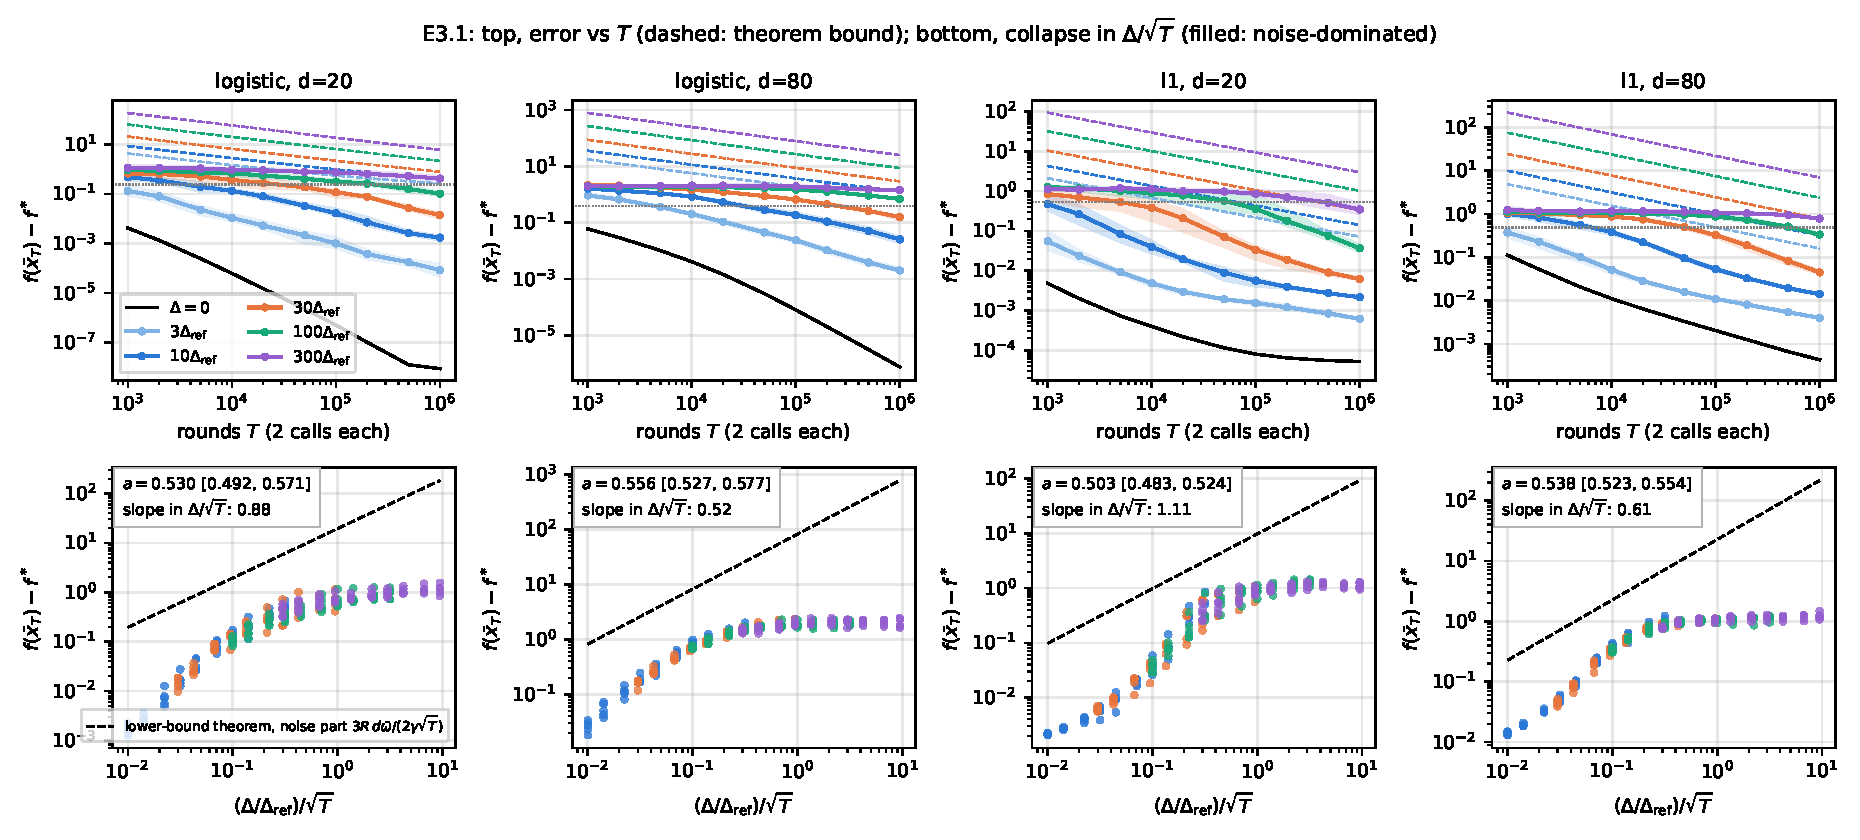
\includegraphics[width=\textwidth]{figs/e31.pdf}
\caption{E3.1. Top: $f(\bar x_T)-f^*$ vs.\ rounds (log--log), geometric mean over 5 runs with min--max band; dashed: the theorem bound $3RG/\sqrt T+2M\gamma$ for each $\Delta$ (same colour); dotted grey: $f(0)-f^*$. Bottom: the same errors against $(\Delta/\Delta_{\rm ref})/\sqrt T$; filled points are noise-dominated; dashed: the noise part of the bound.}\label{fig:e31}
\end{figure}

\textbf{Result.}
\begin{center}\small
\begin{tabular}{@{}lccccc@{}}
\toprule
problem & $a$ (all, 95\% CI) & $\alpha$ & $R^2$ & $a$ (progress only, 95\% CI) & max err/bound\\
\midrule
logistic, $d=20$ & $0.530\ [0.492,0.571]$ & $0.88$ & $0.82$ & $0.524\ [0.476,0.588]$ & $0.107$\\
logistic, $d=80$ & $0.556\ [0.527,0.577]$ & $0.52$ & $0.73$ & $0.521\ [0.476,0.590]$ & $0.089$\\
$\ell_1$, $d=20$ & $0.503\ [0.483,0.524]$ & $1.11$ & $0.86$ & $0.492\ [0.458,0.527]$ & $0.251$\\
$\ell_1$, $d=80$ & $0.538\ [0.523,0.554]$ & $0.61$ & $0.74$ & $0.524\ [0.495,0.572]$ & $0.164$\\
\bottomrule
\end{tabular}
\end{center}
200 noise-dominated points per problem, of which $54$, $24$, $88$ and $43$ (in table order) are in the progress subset; median err/bound in the noise-dominated region $0.036$--$0.067$. \textbf{Verdict.} \emph{Progress subsets:} every CI contains $\frac12$ ($a=0.49$--$0.52$); neither criterion is met. \emph{All points:} the report's criterion is not met (all four $a\in[0.50,0.56]$), but for both $d=80$ problems the CI excludes $\frac12$ (by at most $0.03$), which meets the criterion $a\ne\frac12$ fixed before the study. Most of the all-points sets are saturated points at large $\Delta/\sqrt T$, where the iterate wanders on the sphere $\norm x=R-\gamma$ and the error stops depending on $(\Delta,T)$; these points carry no information on $a$ and dominate the all-points fits. We therefore state the result as: \textbf{collapse in $\Delta/\sqrt T$ confirmed numerically on the progress subsets of the four main problems}; the all-points fits for $d=80$ exclude $\frac12$ by a small margin. The local exponent $\alpha$ of the error in $\Delta/\sqrt T$ is not universal ($0.5$--$1.1$ overall, $1.3$--$2.0$ in the progress region): the collapse curve is not a power law, as expected (worst-case bound: slope 1; strongly convex regime: slope 2). The bound holds everywhere and is conservative by $\approx15$--$25\times$ for these smooth or sharp problems; the ``constant close to 3.1'' is therefore an upper envelope, not a fit.

\textbf{Sensitivity} ($d=20$, $T\le2\cdot10^5$; Fig.~\ref{fig:e31s}). Another logistic instance: $a=0.560\ [0.498,0.629]$, progress-only $0.488\ [0.456,0.525]$. $\gamma\times2$: $0.490\ [0.453,0.531]$. $\ell_1$ with $\gamma\times5$: $0.487\ [0.444,0.515]$. $\pm1$ hash noise (the H3.2 construction; naive ZO-SGD, no decoding): $a=0.671\ [0.558,0.832]$ with a poor fit ($R^2=0.56$, $\alpha=0.32$): \textbf{this variant meets the report's own refutation criterion} ($a\notin[0.4,0.6]$, CI excludes $\frac12$); the progress-only fit has 10 points and is unusable. This variant has the largest $\wbar$ ($\sqrt2\Delta$ vs.\ $0.53\Delta$), hence the largest share of saturated points.

\textbf{Equal-$\wbar$ rerun (added after the first version of this report; not blind: this configuration had already been run when its setup was written).} \emph{Setup:} the $\pm1$ variant with every level multiplied by $\sqrt{2/7}/\sqrt2=0.378$, so that $\wbar$ equals that of the Beta runs at the nominal levels; same seeds as the $\pm1$ variant (common random numbers), $T\le2\cdot10^5$, 5 runs, $24$\,s. \emph{Prediction:} if saturation causes the anomaly, $a\in[0.4,0.6]$ with a CI containing $\frac12$. \emph{Refutation:} as for E3.1. \emph{Result} (Fig.~\ref{fig:e31pm1}; bootstrap with a separate generator): all points $a=0.516\ [0.472,0.566]$ ($160$ points, $\alpha=0.68$, $R^2=0.77$); progress subset $a=0.628\ [0.516,0.772]$ ($29$ points, $R^2=0.89$). \emph{Verdict:} on all points the criterion is not met, so saturation explains most of the anomaly; the progress subset, small as it is, formally meets the refutation criterion. For the $\pm1$ noise with naive ZO-SGD the $\sqrt T$ collapse is therefore \emph{not} established. A possible reason, not tested: with $\pm1$ noise half of the pairs have exactly zero noise difference, so the per-round noise is a two-point mixture rather than a continuous law, and the error need not depend on $(\Delta,T)$ through $\wbar^2/T$ alone. This noise is decodable (Prop.~\ref{prop:pm1}) and is not used as a hard instance.

\begin{figure}[h]\centering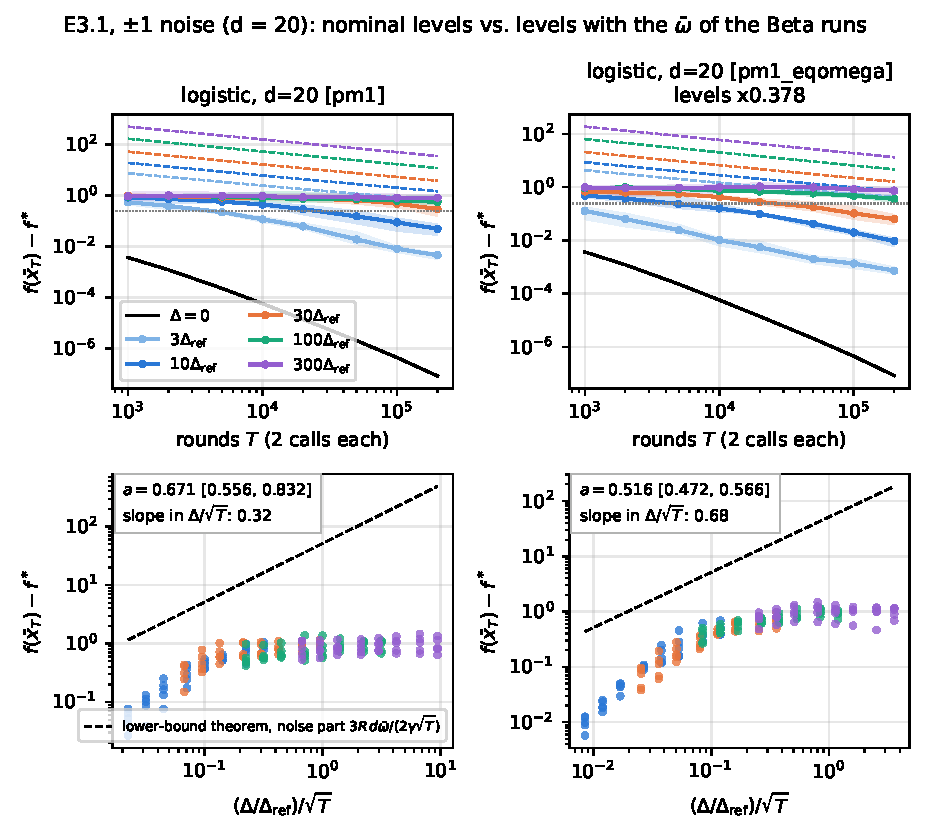
\includegraphics[width=0.62\textwidth]{figs/e31_pm1_eqomega.pdf}
\caption{E3.1, $\pm1$ noise ($d=20$, logistic): left, the sensitivity variant at nominal levels; right, the equal-$\wbar$ rerun (levels $\times0.378$). Same conventions as Fig.~\ref{fig:e31}; the x-axis of the bottom row uses the actual level $\Delta/\Delta_{\rm ref}$, and the dashed line uses the $\wbar$ of the $\pm1$ noise.}\label{fig:e31pm1}
\end{figure}

\begin{figure}[h]\centering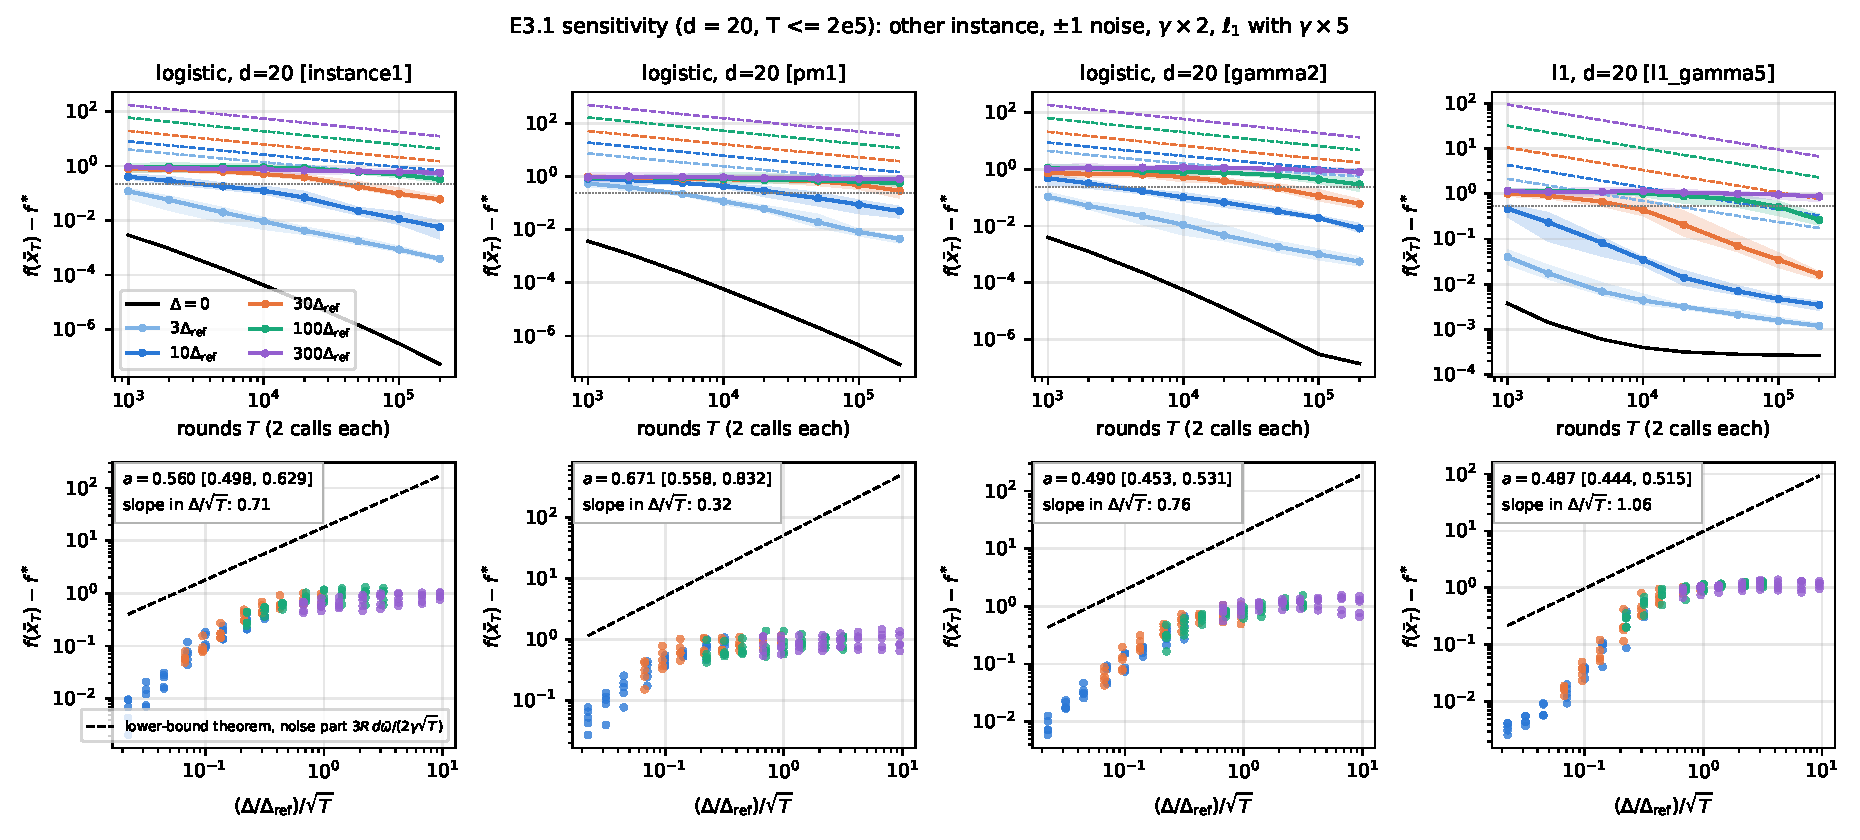
\includegraphics[width=\textwidth]{figs/e31_sensitivity.pdf}
\caption{E3.1 sensitivity: another instance, $\pm1$ noise, $\gamma\times2$, $\ell_1$ with $\gamma\times5$ ($d=20$, $T\le2\cdot10^5$). Same conventions as Fig.~\ref{fig:e31}; the dashed line in the bottom row uses the $\wbar$ of each noise.}\label{fig:e31s}
\end{figure}

\subsection{E3.2: smooth versus rough noise}\label{sec:e32}
\textbf{(a) Estimator level.} \emph{Setup.} $\gamma=\Delta=1$, $d\in\{20,80\}$, 28 log-spaced $\ell/\gamma\in[10^{-2},10^{2.5}]$, $5\times2\cdot10^5$ samples per point. \emph{Prediction} (exact, no free parameter, Lemma~\ref{lem:sin}): $\E\norm n^2/(d^2\Delta^2/4\gamma^2)=1-\Phi_d(2\gamma/\ell)$. \emph{Refutation:} deviations beyond MC error. \emph{Result.} Maximal relative deviation $0.49\%$ ($d=20$) and $0.62\%$ ($d=80$); maximal $\abs z=2.8$ and $3.4$ over 28 points each. The second value is borderline for 56 tests (the pooled standard error of a mean of squares with heavy tails is itself noisy); the identity behind the prediction is checked independently by quadrature to $10^{-14}$ (V8). \emph{Verdict:} confirmed. The prediction $\min\{1,(\gamma/\ell)^2\}$ of the formulation of the hypothesis is off by a factor $\approx d/2$ for $\ell\gtrsim\gamma$ (Fig.~\ref{fig:e32}, left).

\textbf{(b) Optimisation level.} \emph{Setup.} Logistic, $\gamma=0.05$, $\Delta=30\Delta_{\rm ref}$, $T=10^5$, 5 runs; one common step (tuned to the rough limit $\wbar=\Delta$) for all $\ell$; cost $:=$ (error $-$ noiseless error) / (same at $\ell=0.01\gamma$). \emph{Prediction:} cost $\approx1-\Phi_d(2\gamma/\ell)$, within a factor 2 where $\ge0.05$. \emph{Refutation (the formulation of the hypothesis):} cost independent of $\ell$.
\begin{center}\footnotesize\setlength{\tabcolsep}{3pt}
\begin{tabular}{@{}lccccc@{}}
\toprule
$\ell/\gamma$ & $0.1$ & $0.3$ & $1$ & $3$ & $\ge10$\\
\midrule
$d=20$: measured [CI] & $1.32\ [1.08,1.64]$ & $0.73\ [0.68,0.80]$ & $0.18\ [0.12,0.23]$ & $0.019\ [0.009,0.031]$ & $\le0.002$\\
\quad theory $1-\Phi_{20}$ & $1.00$ & $0.69$ & $0.096$ & $0.011$ & $\le0.001$\\
$d=80$: measured [CI] & $1.12\ [1.08,1.16]$ & $0.77\ [0.67,0.87]$ & $0.068\ [0.054,0.081]$ & $0.004\ [0.000,0.009]$ & $\le0.001$\\
\quad theory $1-\Phi_{80}$ & $0.92$ & $0.24$ & $0.025$ & $0.003$ & $0.000$\\
\bottomrule
\end{tabular}
\end{center}
\emph{Verdict.} The refutation criterion of the formulation of the hypothesis is not met: the cost falls by three orders of magnitude between $\ell=0.1\gamma$ and $\ell=10\gamma$. At $\ell=\gamma$ the measured cost is $0.18$ ($d=20$) and $0.068$ ($d=80$), against $1$ predicted by $\min\{1,(\gamma/\ell)^2\}$: that prediction is refuted. The pre-registered factor-2 agreement with $1-\Phi_d$ holds for $d=20$ (worst ratio $1.9$ at $\ell=\gamma$) but fails for $d=80$ at $\ell=0.3\gamma$ ($\times3.2$) and $\ell=\gamma$ ($\times2.8$). A design flaw explains at least part of this: at $\Delta=30\Delta_{\rm ref}$, $T=10^5$ the rough-limit error is saturated ($1.08$ vs.\ $f(0)-f^*=0.40$ for $d=80$; $0.258$ vs.\ $0.241$ for $d=20$), so excess errors are compressed towards the reference and the ratio is not proportional to the excess second moment. A second, unexplained sign points the same way: at $\ell=0.1\gamma$ the normalised cost exceeds $1$ with CIs excluding $1$ ($1.32\ [1.08,1.64]$ for $d=20$, $1.12\ [1.08,1.16]$ for $d=80$), while the second-moment theory gives $1.00$ and $0.92$. So in this design the excess optimisation error is not a function of the excess second moment $\E\norm n^2$ alone; we did not investigate why. The estimator-level law (a) is the clean test; the optimisation-level knee position for $d=80$ remains open. Side result: Beta hash noise with the same $\wbar$ as the rough sinusoid gives the same error ($0.255$ vs.\ $0.258$ for $d=20$; $1.23$ vs.\ $1.08$ for $d=80$), consistent with $\wbar$ being the parameter that matters (Cor.~\ref{cor:osc}).
\begin{figure}[h]\centering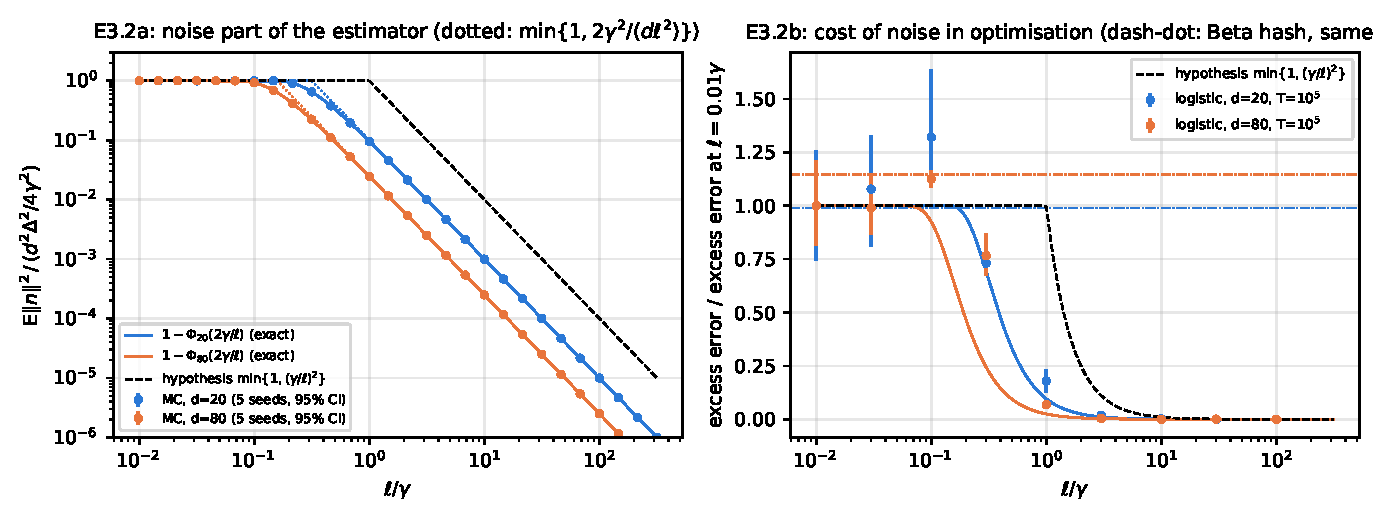
\includegraphics[width=\textwidth]{figs/e32.pdf}
\caption{E3.2. Left: normalised $\E\norm n^2$ vs.\ $\ell/\gamma$ (log--log); dots: MC with 95\% CI; solid: exact $1-\Phi_d(2\gamma/\ell)$; dotted: $\min\{1,2\gamma^2/(d\ell^2)\}$; dashed black: the hypothesis $\min\{1,(\gamma/\ell)^2\}$. Right: excess optimisation error normalised at $\ell=0.01\gamma$ (mean, 95\% bootstrap CI over runs); solid: $1-\Phi_d$; dash-dot: Beta hash noise with the same $\wbar$.}\label{fig:e32}
\end{figure}

\subsection{E3.3: one-point methods versus two-point methods (not run)}\label{sec:e33}
A faithful test needs an implementation of a kernel-based one-point method (Lattimore--Gy\"orgy; Fokkema et al.); this did not fit the available resources. What was done instead: (i) the rigorous ingredients Props.~\ref{prop:any}, \ref{prop:ballavg} and Cor.~\ref{cor:cross}; (ii) the analytic comparison of Fig.~\ref{fig:e33}, which plots the proven two-point bracket, the bandit formula $d^{-k/2}$ (with $C_b=1$, an assumption) and the universal upper bound, in units of $\varepsilon\sqrt T$. The bandit curves are the range-normalised guarantee $\Delta_{\rm band}(T)$ of Cor.~\ref{cor:cross}, drawn at the budgets $T=64\,d^k(MR/\varepsilon)^2$ and $256\,d^k(MR/\varepsilon)^2$ (i.e.\ $64d^{k-1}T_0$ and $256d^{k-1}T_0$; $C_b=1$); at $T\le16d^{k-1}T_0$, which contains every complexity-preserving budget $CT_0$ with $C\le16d^{k-1}$, they are identically zero. With $C_b=1$ the crossover with the two-point upper bound for $d=20$, $k=3$ is at $MR/\varepsilon\approx128\pi\sqrt{20}\approx1.8\cdot10^3$ at the larger budget, rather than $\sqrt d$; the position of the crossover is therefore a statement about constants nobody has computed. \textbf{Run plan.} Implement the one-point kernel method of Lattimore--Gy\"orgy 2023 (or the simpler ellipsoid variant of Fokkema et al.\ 2024) with ball averaging (Prop.~\ref{prop:ballavg}); quadratic and $\ell_1$ objectives, $d\in\{10,20,40\}$, $MR/\varepsilon\in\{2,5,10,30,100\}$, the cell noise of Def.~\ref{def:noise} at $\Delta\in\{10,30,100\}\Delta_{\rm ref}$; measure $\Delta_{50}(T)$ for both methods and the crossover in $MR/\varepsilon$. Refutation as pre-registered: no crossover.
\begin{figure}[h]\centering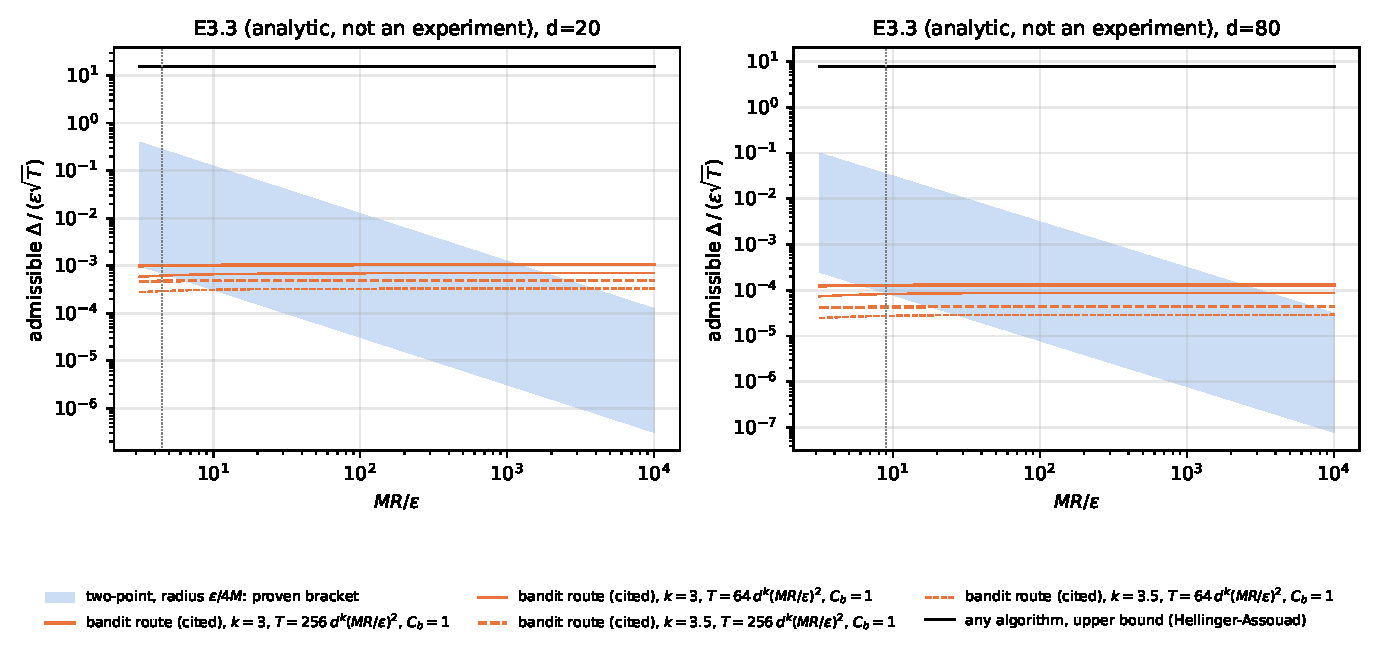
\includegraphics[width=\textwidth]{figs/e33_analytic.pdf}
\caption{E3.3 (analytic, not an experiment). Admissible $\Delta/(\varepsilon\sqrt T)$ vs.\ $MR/\varepsilon$ for $\gamma=\varepsilon/(4M)$. Blue band: proven bracket for $\Atwo$ (Thm.~\ref{thm:main}); orange: range-normalised bandit guarantee $\Delta_{\rm band}$ of Cor.~\ref{cor:cross} at $T=256\,d^k(MR/\varepsilon)^2$ (thick) and $64\,d^k(MR/\varepsilon)^2$ (thin), $C_b=1$, cited rates not re-checked; it vanishes for $T\le16d^k(MR/\varepsilon)^2$; black: upper bound for any algorithm (Prop.~\ref{prop:any}); dotted: $MR/\varepsilon=\sqrt d$.}\label{fig:e33}
\end{figure}

\subsection{E3.4 (new): the hard instance against ZO-SGD}\label{sec:e34}
\textbf{Setup.} $f_v=a\ip vx$ on $B_1$, Beta hash noise ($I=10$), $\Delta=1$, $\gamma=0.01$, $d\in\{20,80\}$, $T\in\{10^3,10^4,10^5\}$, $a=a^*\times\{\frac1{16},\frac14,1,4,16\}$ with $a^*=\sqrt d\Delta/(4\gamma\sqrt{IT})$; 20 runs (5 seeds $\times$ 4 random $v$) per cell; step scale $\in\{0.1,1,10\}$, the best one reported (each step scale is a single algorithm of $\Atwo$, so the minimum of their risks is still bounded below). \textbf{Prediction.} Lemma~\ref{lem:assouad} with Thm.~\ref{thm:upper}'s estimates: mean error $\ge LB(a)=\frac{aR}{4\sqrt d}(d-2\gamma a\sqrt{dIT}/\Delta)_+$. \textbf{Refutation.} Mean error (upper end of its 95\% CI) below $LB$. \textbf{Result.} Never refuted: the smallest ratio (lower CI end)$/LB$ is $3.7$; at $a=a^*$ the ratio is $5.9$--$6.6$ in all six $(d,T)$ cells. In units of $a^*R\sqrt d$ the curves for different $T$ coincide (Fig.~\ref{fig:e34}), as the scaling $a^*\propto\sqrt d\Delta/(\gamma\sqrt T)$ predicts. \textbf{Verdict: a sanity check only.} The test cannot fail for a method that learns nothing, since $LB(a)\le aR\sqrt d/4$ is below the trivial error $aR\sqrt d$ of the output $\hat x=0$; and indeed for $a\le a^*$ ZO-SGD stays at $0.79$--$1.00$ of the trivial error. The ratio $\approx6$ at $a^*$ reflects the factor $\frac18$ of the Assouad bound relative to the trivial error, not near-tightness of $32\pi$. ZO-SGD reaches the relative accuracy $\frac18$ that the bound certifies at $a^*$ only around $a\approx16a^*$ (error/trivial $0.11$--$0.18$). E3.4 is not counted as support for H3.2a.
\begin{figure}[h]\centering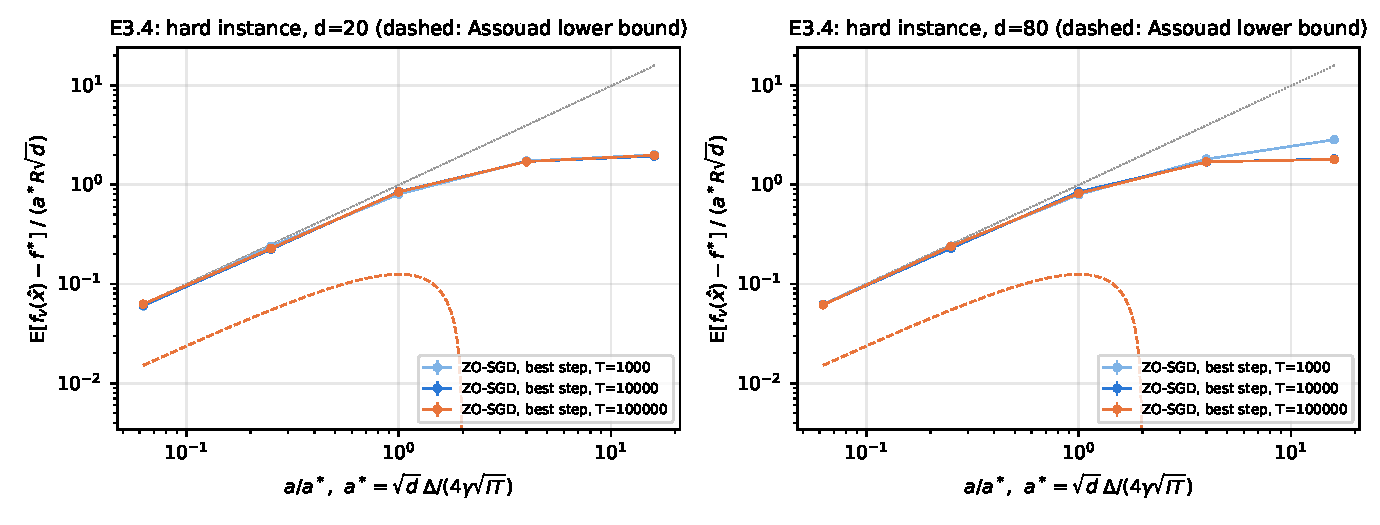
\includegraphics[width=\textwidth]{figs/e34.pdf}
\caption{E3.4. Mean error of ZO-SGD (best of 3 steps; 95\% CI over 20 runs) on the hard instance vs.\ $a/a^*$, in units of $a^*R\sqrt d$; dashed: the Assouad lower bound (it vanishes for $a\ge2a^*$, where the Lipschitz cap is not binding); dotted: the line $y=x$, the trivial error of the starting point $\hat x=0$.}\label{fig:e34}
\end{figure}

\subsection{E3.5 (new): the $\pm1$ noise is decodable}\label{sec:e35}
\textbf{Setup.} Logistic, $d=20$, $\gamma=0.05$, $\Delta/\Delta_{\rm ref}\in\{10,100\}$ (here $2M\gamma=8.94\Delta_{\rm ref}$), $T=10^5$, 5 runs; arms: noiseless; $\pm1$ hash noise decoded by $g=D-2\Delta\,\mathrm{round}(D/2\Delta)$ (same direction stream as the noiseless arm); $\pm1$ raw; Beta noise raw with the same $\Delta$. \textbf{Prediction} (Prop.~\ref{prop:pm1}): decoded $=$ noiseless to rounding error. \textbf{Result.} Maximal difference of the recorded errors $1.7\cdot10^{-16}$; final errors: noiseless and decoded $4.2\cdot10^{-7}$; raw $\pm1$: $0.10$ and $0.79$; raw Beta: $0.014$ and $0.46$. \textbf{Verdict.} Confirmed. The construction of H3.2 as written defeats ZO-SGD but, for $\Delta>2M\gamma$, not an algorithm of the same class with one extra line; our upper bound therefore uses a law with finite Fisher information instead (whether such a law is necessary at $\Delta\le2M\gamma$ is not shown).
\begin{figure}[h]\centering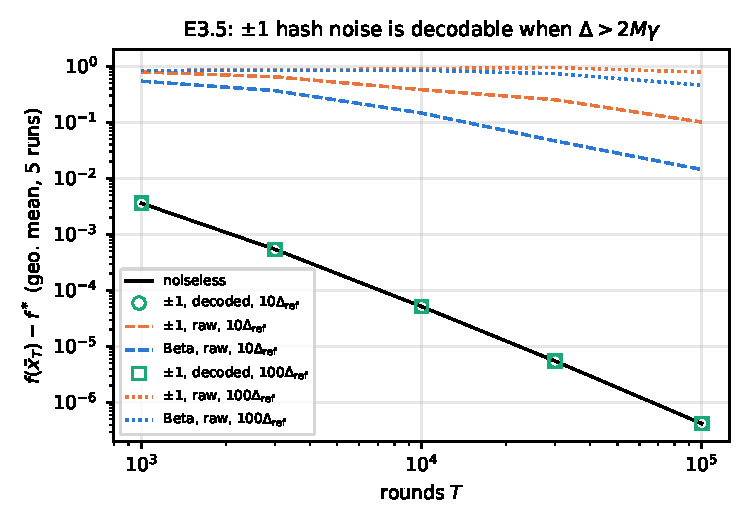
\includegraphics[width=0.62\textwidth]{figs/e35.pdf}
\caption{E3.5. Error vs.\ rounds (geometric mean of 5 runs). Hollow markers (decoded $\pm1$ noise) lie exactly on the noiseless curve.}\label{fig:e35}
\end{figure}

%==========================================================================================
\section{Verdict}\label{sec:verdict}
{\small
\begin{xltabular}{\textwidth}{@{}>{\raggedright\arraybackslash}p{5.3cm}>{\raggedright\arraybackslash}p{4.6cm}>{\raggedright\arraybackslash}X@{}}
\toprule
Claim & Status & Support\\
\midrule
\endhead
H3.1a ZO-SGD (batch 1, idle in round 1) is $\varepsilon$-accurate for $\wbar/2\le\Dlow(T)$, explicit constants & proven under a condition (i.i.d.\ states with arbitrary initial law, one idle round --- or stationary start without it; convex $M$-Lipschitz $f$, $\gamma+\rho\le\varepsilon/(4M)$; expectation; probability with $\varepsilon\to\beta\varepsilon$) & Lemma~\ref{lem:mom}, Thm.~\ref{thm:lower}, Cor.~\ref{cor:lower}, Remark~\ref{rem:lower}(vi); V11, V17; E3.1 (bound holds, max ratio 0.25)\\
H3.1b $\Dcp^E(24)\ge1.034M\gamma/\sqrt d$ for $\tau=1$ (expectation variant; probability variant at $C=24/\beta^2$) & proven (same conditions, $\varepsilon<MR/8$) & Cor.~\ref{cor:lower}(b); V15\\
H3.1c consistency with the heuristic threshold ($\xi\equiv0$, $b=1$ gives $M\gamma/\sqrt d$) & consistency check (informal) & Remark~\ref{rem:lower}(i)\\
H3.2a $\Dmax^{E,\mathrm{2pt},\gamma}\le32\pi\varepsilon\gamma\sqrt T/(dR)$ & proven for $\Atwo$ (non-adaptive direction laws), $\varepsilon<MR/8$ & Lemmas~\ref{lem:inclass}--\ref{lem:couple}, Thm.~\ref{thm:upper}; V1, V3--V7 (E3.4 is a sanity check only)\\
H3.2b same for adaptive direction laws & remains a hypothesis & Remark~\ref{rem:scope}(i)\\
H3.2c two-sided $\Theta(\varepsilon\gamma\sqrt T/(dR))$ & proven for $\Atwo$ under the conditions of Thm.~\ref{thm:main} (convex $M$-Lipschitz $f$, $\gamma\le\varepsilon/(4M)$; the smooth class with $\gamma>\varepsilon/(4M)$ not covered) & Thm.~\ref{thm:main}, Remark~\ref{rem:scope}(iv); E3.1 (collapse on the progress subsets)\\
H3.2d the $\pm1$ cell noise gives an upper bound & refuted for $\Delta>2M\gamma$ (any $f$) and for the linear hypercube family at every $\Delta$; open for other families at $\Delta\le2M\gamma$ & Prop.~\ref{prop:pm1}; V13; E3.5\\
H3.3a any algorithm: $\Dmax^E\le16\sqrt2\pi\varepsilon\sqrt T/\sqrt d$ & proven & Prop.~\ref{prop:any}\\
H3.3b bandit methods beat two-point ones for $MR/\varepsilon\gtrsim\sqrt d$ & proven under a condition: Assumption (B$_k$) (cited rates for losses in $[0,1]$, not re-checked, $C_b$ unknown), budget $T\ge2+256C_bd^{k-1}T_0$, and $MR/\varepsilon>128\pi\sqrt{C_b}d^{k/2-1}$ ($\sqrt d$ for $k=3$, $d^{3/4}$ for $k=3.5$) & Cor.~\ref{cor:cross}; V16; E3.3 not run. For $T\le2+16C_bd^{k-1}T_0$ (every complexity-preserving budget $CT_0$ with $C\le16C_bd^{k-1}$) the cited rates give no guarantee\\
H3.3c fixed-$\gamma$: the Bessel part blocks bandit methods & refuted (information-theoretically) & Prop.~\ref{prop:ballavg}\\
H3.3d all-radii class: true threshold $=$ max of the two formulas & remains a hypothesis (lower side conditional, upper gap $d^{(k-1)/2}$) & Cor.~\ref{cor:cross}\\
H3.4a noise part $\le d\omega_\delta/(2\gamma)$; bounds in terms of $\omega_\delta/2$ and $\wbar/2$ & proven & Lemma~\ref{lem:osc}, Cor.~\ref{cor:osc}\\
H3.4b $\Lambda$-Lipschitz noise costs $M\to M+\Lambda$ & proven & Cor.~\ref{cor:lip}; V12\\
H3.4c smooth noise: cost $\propto1-\Phi_d(2\gamma/\ell)$, knee at $\gamma/\sqrt d$ (refines ``$\min\{1,\gamma/\ell\}^2$'') & proven (estimator); confirmed numerically (E3.2a); optimisation level: confirmed for $d=20$, not for $d=80$ & Lemma~\ref{lem:sin}; V8; E3.2\\
H3.4d rounding: $\omega_\delta\le u$, $\wbar\le u/2$, tie $=$ signal erased & proven (uniform fresh offset only) & Prop.~\ref{prop:round}; V10\\
E3.1 collapse in $\Delta/\sqrt T$ & confirmed numerically on the progress subsets of the four main problems; all-points fits for $d=80$ exclude $\frac12$ (by $\le0.03$); the $\pm1$ variant meets the refutation criterion, mostly explained by saturation (equal-$\wbar$ rerun), progress subset of the rerun still anomalous & \S\ref{sec:e31}; Fig.~\ref{fig:e31pm1}\\
Remark on $T\ll T_0$ and H2's second branch (earlier version of this report: ``$\Delta=0$ unsolvable, branch vacuous'') & withdrawn (citation did not apply) & Remark~\ref{rem:scope}(iii)\\
\bottomrule
\end{xltabular}}

%==========================================================================================
\section{Implications}\label{sec:contrib}
\subsection{For the general problem}
\begin{enumerate}
\item The expected picture $\Delta^{\rm adv}_{\max}\lesssim\Dcp(C)\lesssim M\gamma/\sqrt d$ is now proven on both sides for $\tau=1$ \emph{for two-point methods of radius $\gamma$} and convex $M$-Lipschitz $f$ with $\gamma\le\varepsilon/(4M)$. Two separate statements: the \emph{lower side} (Cor.~\ref{cor:lower}(b), proven) $\Dcp^{E,\mathrm{2pt},\gamma}(24)\ge1.034M\gamma/\sqrt d$ in the expectation variant, and $\Dcp(24/\beta^2)\ge1.034M\gamma/\sqrt d$ in the probability variant; the \emph{upper side} (Thm.~\ref{thm:upper}, proven for $\Atwo$) at $T=CT_0=CdM^2R^2/\varepsilon^2$: $\Dcp^{E,\mathrm{2pt},\gamma}(C)\le32\pi\,\varepsilon\gamma\sqrt{CT_0}/(dR)=32\pi\sqrt C\,M\gamma/\sqrt d$ for $\varepsilon<MR/8$, and $\Dcp^{\mathrm{2pt},\gamma}(C)\le64\pi\sqrt C\,M\gamma/\sqrt d$ in the probability variant for $\beta\le1/32$, $\varepsilon<MR/16$. The upper side is what closes H1.5d for $\tau=1$ and $\Atwo$.
\item For arbitrary query points our bounds do not characterise the threshold: they leave a gap up to $\asymp\sqrt d\,MR/\varepsilon$ between $\Dlow$ and $71\varepsilon\sqrt T/\sqrt d$ (Prop.~\ref{prop:any}, proven). The cited bandit rates, rescaled to the range of $f$, exceed the two-point upper bound only at budgets $T\gtrsim C_bd^{k-1}T_0$ and for $MR/\varepsilon\gtrsim d^{k/2-1}$ (proven under Assumption (B$_k$)); at complexity-preserving budgets $T\asymp CT_0$ they give no guarantee and do not beat two-point methods (Cor.~\ref{cor:cross}). The value of $\Dmax$ therefore depends on the algorithm class it refers to: for $\Atwo$ at $\tau=1$, under the conditions of Thm.~\ref{thm:main} (convex $M$-Lipschitz $f$ on $B_R$, arbitrary initial law, $\varepsilon<MR/8$, $\gamma\le\varepsilon/(4M)$, $T\ge1+16d^2M^2R^2/((d-1)\varepsilon^2)$), it is $\Theta(\varepsilon\gamma\sqrt T/(dR))$; for all algorithms it is only bracketed.
\item The noise parameter of the two-point problem is the (mean-square) oscillation on scale $2\gamma$, not the amplitude: $\Delta$ may be replaced by $\omega_\delta(2\gamma)/2$ in every bound of this report for two-point methods (Cor.~\ref{cor:osc}, proven).
\end{enumerate}

\subsection{For the other hypotheses}
\textbf{H2:} first branch at $\tau=1$ proven from both sides for $\Atwo$ (it was proven from below only, with burn-in, in H1); nothing is concluded about the second branch $\sqrt{\ln T/d}$ (Remark~\ref{rem:scope}(iii)). \textbf{H5:} the upper-bound machinery (Hellinger, sequential BC, coupling with an idealised oracle) is expected to apply to the false-valley construction (not checked here); the $\pm1$ lesson applies to H5.1--5.2 as well: two-valued noise inside a state can be decodable (at least for $\Delta>2M\gamma$, Prop.~\ref{prop:pm1}), so our technique would give anti-states a noise law with finite Fisher information. \textbf{H4:} its $\tau=1$ base case is Thm.~\ref{thm:lower}. \textbf{H6:} unchanged; Prop.~\ref{prop:ballavg} shows that \emph{any} algorithm can neutralise the Bessel part by averaging over the class radius, so H6 is a statement about methods that cannot (or do not) do this. \textbf{H7, H10:} rounding with a fresh offset is $\tau=1$ noise with $\wbar\le u/2$ (Prop.~\ref{prop:round}, proven for a uniform fresh offset); H10's shared dither is exactly this regime. Rounding with a method-driven offset (H8) is not covered.

\subsection{Open questions}
\begin{enumerate}
\item \emph{Algorithm class.} For algorithms with arbitrary query points and individual values, is the threshold at $\tau=1$ and $T\asymp CT_0$ larger than that of two-point methods? Our bracket there is $[\Dlow,\,71\varepsilon\sqrt T/\sqrt d]$.
\item \emph{Adaptive direction laws.} Does Thm.~\ref{thm:upper} extend to methods that choose their direction law adaptively (H3.2b, remains a hypothesis)?
\item \emph{Constants and scope.} The two sides differ by the factor $128\pi$; the lower side does not cover the smooth class with $\varepsilon/(4M)<\gamma\le\sqrt{\varepsilon/L}$.
\item \emph{Two-valued noise.} Is some two-valued noise hard at the complexity-preserving levels $\Delta\lesssim\sqrt C M\gamma/\sqrt d<2M\gamma$, or is a law with finite Fisher information necessary?
\item \emph{Numerics.} E3.3 (one-point versus two-point methods) was not run; the optimisation-level knee of E3.2 for $d=80$ and the residual anomaly of the $\pm1$ noise on the progress subset of the equal-$\wbar$ rerun are unresolved.
\end{enumerate}

%==========================================================================================
\appendix
\section{Verification checks}\label{app:checks}
\begin{center}\small
\begin{tabularx}{\textwidth}{@{}lXl@{}}
\toprule
ID & Check & Outcome\\
\midrule
V1 & Fisher information and normalisation: $I(\cos^2(\pi t/2))=\pi^2$, $I(\frac{15}{16}(1-t^2)^2)=10$ (sympy) & exact\\
V2 & $\mathrm{Var}=\frac13-\frac2{\pi^2}$ and $\frac17$ (sympy) & exact\\
V3 & $H^2(p_b,p)\le b^2I/4$, both densities, $b\in[10^{-3},1]$ (quadrature) & max ratio $0.9997$\\
V4 & same for the law of $U-U'$ (Beta case; data processing) & ratios $0.34$--$0.36$\\
V5 & hash noise: KS vs.\ $\mathrm{Beta}(3,3)$, pair independence, no pair in one cell ($10^5$ pairs) & $p=0.07$, corr $7.7\cdot10^{-4}$, 0 pairs\\
V6 & $\sqrt d-\sqrt{d-i}\ge i/(2\sqrt d)$ ($d<400$); separation lemma on random points & pass, min slack $4\cdot10^{-10}$\\
V7 & sequential BC bound and $\TV\le\sqrt{1-\BC^2}$, 200 random adaptive two-round designs (exact) & pass\\
V8 & $\E\sin^2(\kappa e_1)=\frac12(1-\Phi_d(2\kappa))$, $d\in\{3,20,80\}$ & error $10^{-14}$\\
V9 & $\sqrt6-\sqrt{d/(d-1)}\ge1$ for $2\le d\le10^4$; constants $32\pi$, $32\sqrt{10}$, $16\sqrt2\pi$ & min $1.035$\\
V10 & rounding with uniform offset: tie law, $\E(D\delta)^2=u^2r'(1-r')$, $\abs{D\delta}\le u$ & pass ($4\cdot10^5$ samples)\\
V11 & $\E\norm Y^2\le G^2$ (logistic, Beta noise, $\Delta=30\Delta_{\rm ref}$) & ratio $0.79$\\
V12 & Lipschitz-noise bound $d^2(M+\Lambda)^2/(d-1)$ & $51\le276$\\
V13 & $\pm1$ decoder exact for $\abs g<\Delta$ & pass\\
V14 & $I(U-U')\le I(U)$ (Beta) & $3.63\le10$\\
V15 & Cor.~\ref{cor:lower}(b) with the idle round: $\varepsilon\sqrt{24T_0-1}/(2R)=\sqrt dM\sqrt{6(1-1/(24T_0))}$ (sympy); factor $\ge1.034$ for $T_0>64d$, $2\le d\le10^4$ & min $1.0349$ ($d=2$)\\
V16 & Cor.~\ref{cor:cross}: $\Delta_{\rm band}$ solved from the budget (sympy); both crossovers; clean form of (b) on a grid & pass\\
V17 & round-1 bias of Remark~\ref{rem:lower}(vi), $d\in\{20,80\}$, $2\cdot10^5$ samples, vs.\ $\frac d\gamma\Delta\E\abs{e_1}$ & within $4$ s.e.\\
\bottomrule
\end{tabularx}
\end{center}
The checks V1--V17 take about 4\,s; all runs together take about 50 min on one CPU core. Figures and statistics are computed from the stored raw results only.

\textbf{What was not checked.} The cited bandit theorems (statements, constants); adaptive direction laws; $\tmix\le1$ chains that are not i.i.d.\ (only via H1 Cor.~4.17); dimensions above $80$; E3.3; the optimisation-level knee of E3.2 for $d=80$ (saturated design) and the E3.2b costs above $1$; the residual anomaly of the $\pm1$ noise on the progress subset of the equal-$\wbar$ rerun. Reproducibility: with fixed seeds the logistic runs reproduce to $10^{-10}$, but the $\ell_1$ runs are reproducible only statistically, not bitwise (a repeated run found individual $\ell_1$, $d=80$ runs at low levels differing by up to $42\%$, with per-level geometric means within about $10\%$; likely floating-point non-determinism in the LP solution or BLAS, amplified by the nonsmooth objective).
\end{document}
